%\documentclass[12pt,draftcls]{ucdavisthesis}
\documentclass[12pt]{ucdavisthesis}

% PLEASE READ THE MANUAL - ucdavisthesis.pdf (in the package installation directory)

%%%%%%%%%%%%%%%%%%%%%%%%%%%%%%%%%%%%%%%%%%%%%%%%%%%%%%%%%%%%%%%%%%%%%%%%
%                                                                      %
%               LATEX COMMANDS FOR DOCUMENT SETUP                      %
%                                                                      %
%%%%%%%%%%%%%%%%%%%%%%%%%%%%%%%%%%%%%%%%%%%%%%%%%%%%%%%%%%%%%%%%%%%%%%%%

%\usepackage{bookmark}
\usepackage[us,nodayofweek,12hr]{datetime}
\usepackage{graphicx}
%\usepackage[square,comma,numbers,sort&compress]{natbib}
%\usepackage{hypernat}
% Other useful packages to try
%\usepackage{amsmath}
%\usepackage{amssymb}
%
% Different fonts to try (uncomment only fontenc and one font at a time)
% (you may need to install these first)
%\usepackage[T1]{fontenc} %enable fontenc package if using one of the fonts below
%\usepackage[adobe-utopia]{mathdesign}
%\usepackage{tgschola}
%\usepackage{tgbonum}
%\usepackage{tgpagella}
%\usepackage{tgtermes}
%\usepackage{fourier}
%\usepackage{fouriernc}
%\usepackage{kmath,kerkis}
%\usepackage{kpfonts}
%\usepackage[urw-garamond]{mathdesign}
%\usepackage[bitstream-charter]{mathdesign}
%\usepackage[sc]{mathpazo}
%\usepackage{mathptmx}
%\usepackage[varg]{txfonts}

\hyphenation{dis-ser-ta-tion blue-print man-u-script pre-par-ing} %add hyphenation rules for words TeX doesn't know


%\renewcommand{\rightmark}{\scriptsize A University of California Davis\ldots \hfill Rev.~\#1.0 \quad Compiled: \currenttime, \today}
% a fancier running header that can be used with draftcls options

%%%%%%%%%%%%%%%%%%%%%%%%%%%%%%%%%%%%%%%%%%%%%%%%%%%%%%%%%%%%%%%%%%%%%%%%
%                                                                      %
%        DOCUMENT SETUP AND INFORMATION FOR PRELIMINARY PAGES          %
%                                                                      %
%%%%%%%%%%%%%%%%%%%%%%%%%%%%%%%%%%%%%%%%%%%%%%%%%%%%%%%%%%%%%%%%%%%%%%%%

\title          {A Polyhedral Finite Element Approach to \\ 
                 Image-Based Modeling and Simulation in Biomechanics}
%Exact title of your thesis. Indicate italics where necessary by underlining or using italics. Please capitalize the first letter of each word that would normally be capitalized in a title.

\author         {Omar Mohamed Hafez}
%Your full name as it appears on University records. Do not use initials.

\authordegrees  {B.S. Civil Engineering (University of California, Davis) 2009 \\
                 M.S. Civil Engineering (University of California, Davis) 2010 \\
                 M.S. Applied Mathematics (University of California, Davis) 2012}
%Indicate your previous degrees conferred.

\officialmajor  {CIVIL AND ENVIRONMENTAL ENGINEERING}
%This is your official major as it appears on your University records.

\graduateprogram{Civil and Environmental Engineering}
%This is your official graduate program name. Used for UMI abstract.

\degreeyear     {2017}
% Indicate the year in which your degree will be officially conferred.

\degreemonth    {December}
% Indicate the month in which your degree will be officially conferred. Used for UMI abstract.

\committee{Mark Rashid}{Committee Member Name}{Committee Member Name}{}{}
% These are your committee members. The command accepts up to five committee members so be sure to have five sets of braces, even if there are empties.

%%%%%%%%%%%%%%%%%%%%%%%%%%%%%%%%%%%%%%%%%%%%%%%%%%%%%%%%%%%%%%%%%%%%%%%%

%\copyrightyear{2017}
%\nocopyright

%%%%%%%%%%%%%%%%%%%%%%%%%%%%%%%%%%%%%%%%%%%%%%%%%%%%%%%%%%%%%%%%%%%%%%%%

\dedication{\textsl{To \ldots}}

%%%%%%%%%%%%%%%%%%%%%%%%%%%%%%%%%%%%%%%%%%%%%%%%%%%%%%%%%%%%%%%%%%%%%%%%

\abstract{The abstract submitted as part of your dissertation, in the introductory pages, does not have a word limit. It should follow the same format as the rest of your dissertation (1.5 inch left margin, double-spaced, consecutive page numbering, etc.).}

%%%%%%%%%%%%%%%%%%%%%%%%%%%%%%%%%%%%%%%%%%%%%%%%%%%%%%%%%%%%%%%%%%%%%%%%

\acknowledgments{Acknowledgements to those who helped you get to this point. They should be listed by chapter when appropriate.}

%%%%%%%%%%%%%%%%%%%%%%%%%%%%%%%%%%%%%%%%%%%%%%%%%%%%%%%%%%%%%%%%%%%%%%%%

% Each chapter can be in its own file for easier editing and brought in with the \include command.
% Then use the \includeonly command to speed compilation when working on a particular chapter.
%%% \includeonly{chap1}

\begin{document}

\newcommand{\bibfont}{\singlespacing}
% need this command to keep single spacing in the bibliography when using natbib

\bibliographystyle{ieeetr}
%many other bibliography styles are available (IEEEtran, mla, etc.). Use one appropriate for your field.

\makeintropages %Processes/produces the preliminary pages

\chapter{Overview}
\textit{Image-based modeling and simulation}, also known as \textit{patient-specific modeling and simulation} or \textit{in-silico modeling and simulation}, is the process of performing mathematical computations based on imaging data to analyze and predict the physical behavior of biological tissues. Imaging data directly provides the geometry and/or material properties of the biological structures of interest, in contrast to conventional engineering disciplines where the geometry and materials of an object originate from man-made designs. Historically, studies of biological tissues or organisms have been limited to either \textit{in vivo} (within the living) experimentation or \textit{ex vivo} (outside of the living) experimentation. \textit{In vivo} studies raise concerns about cost, study controls, and the ethics of experimenting on living beings, while \textit{ex vivo} studies can never truly represent how an organism behaves after it has been removed from its native environment. \textit{In silico} (in silicon) studies provide the ability to model \textit{in vivo} behavior without the same concerns of cost or ethics, and with more control of desired detail than what \textit{ex vivo} affords~\cite{colquitt_2011}. That control allows \textit{in silico} approaches to be used in conjunction with \textit{in vivo} and \textit{ex vivo} ones to advance the medical sciences in a number of exciting ways.

%%%%%

Image-based modeling and simulation has played an important predictive and analytic role in several areas, including:  medical device design optimization,  surgical planning, improved diagnosis and treatment, understanding causes of pathology, computer-assisted surgery, and surgeon training. These technologies have been applied to nearly every area of the body, including: the cardiovascular system~\cite{min_2015, updegrove_2016}, brain~\cite{weickenmeier_2016, behnia_2008}, knee~\cite{erdemir_2015, donahue_2002}, hip~\cite{anderson_2008, el'sheikh_2003}, spine~\cite{malandrino_2014, dumas_2005}, liver~\cite{shi_2008, schwen_2014}, kidney~\cite{eloot_2002, snedeker_2005}, jaw~\cite{idrus_2017, narra_2014}, and teeth~\cite{frisardi_2011, geng_2001}. 

Regulatory organizations and professional societies have identified the burgeoning potential of computational modeling in the medical device field. The American Society of Mechanical Engineers (ASME) and the U.S. Food and Drug Administration (FDA) formed a subcomittee in 2010 named ``V\&V 40: Verification and Validation in Computational Modeling of Medical Devices'', out of which a regulatory standard is expected to be published in early 2018~\cite{committee}. The Center for Devices and Radiological Health (CDRH) at the FDA identified Computational Modeling as a priority in FY2017~\cite{Morrison2017}. The FDA has published several guidelines in the last few years: ``Reporting of Computational Modeling Studies in Medical Device Submissions''~\cite{fda1_2016}, ``Software as a Medical Device (SAMD): Clinical Evaluation''~\cite{fda1_2016}, and ``Applicability Analysis of Validation Evidence for Biomedical Computational Models''~\cite{pathmanathan_2017}. The development of tools and regulations related to \textit{software as a medical device} demonstrates the extent to which industry and regulatory bodies have invested in computational modeling to move healthcare forward. And, \textit{in silico} modeling and simulation lies at the heart of those development efforts.

%%%%%

The field of image-based modeling and simulation covers a broad spectrum of topics, including image processing, computational geometry, numerical methods, and biomechanics. The workflow entails: medical imaging and image segmentation, image-based mesh generation, physics-based modeling and simulation, and use in medical applications. Each of these steps is described in turn. The work described herein outlines novel contributions to certain elements of this workflow, as well as novel combinations of existing technologies.

\chapref{2} describes the basic physics involved in acquiring medical images for a number of imaging modalities. Medical images will be assumed here to be three-dimensional rectilinear grids of \textit{voxels}, or 3D pixels. The chapter also presents a review of current image segmentation techniques, which delimit the voxels in an image into the various objects and tissues of interest. \chapref{3} discusses image-based mesh generation, which involves generating geometrical meshes suitable for simulation based on segmented images. Image-based meshing is often separated into two steps: 1) surface generation,  and 2) conventional CAD-based volume meshing. A novel Voronoi-based surface generation technique is presented, and a brief review of CAD-based meshing techniques is covered. A novel image-based meshing tool \textit{Shabaka} is introduced, that makes important improvements to the speed and robustness of generating meshes from image data.

The next step in the workflow - physics-based modeling and simulation - may refer to a number of different physical phenomena and numerical methods. \chapref{4} presents pertinent theory and implementation specific to modeling nonlinear solid mechanics using finite element methods (FEM). Principles of continuum mechanics and finite element methods are discussed, as well as a particular type of polyhedral finite elements. An implementation of incremental kinematics within finite element codes is presented, and the use of hyperelastic materials in an incremental kinematics framework is demonstrated. \chapref{5} covers the use of image-based modeling and simulation in the field of cardiac mechanics. The important numerical considerations in performing human heart modeling are discussed. Contributions made to an existing cardiac mechanics code are highlighted, and simulation results using that code are shown.

Future work is discussed on several fronts in \chapref{6}. Progress toward demonstrating polyhedral finite element methods as a viable option in human heart modeling is presented. Potential improvements to both the image-based meshing and cardiac mechanics codes are noted. Broader topics in the future of image-based modeling and simulation are also mentioned, specifically how it is playing a role in the \textit{simulation of clinical trials} and in applications in \textit{rapid prototyping} and \textit{additive manufacturing}. A continuing project is discussed that uses machine learning in conjunction with the novel image-based meshing tool introduced in \chapref{3}. Lastly, concluding remarks are given in \chapref{7}.

For the electronic version of this document, images may be enlarged for detail.

\chapter{Medical Imaging}
%
\begin{figure}[tbh]
\centering

\includegraphics{media/ucdavisthesis_example_figure}
% where an .eps filename suffix will be assumed under latex,
% and a .pdf suffix will be assumed for pdflatex
\caption[First sample figure]{A sample figure.}
\label{fig.sample_1}
\end{figure}

\section{Magnetic Resonance Imaging}
\label{Magnetic Resonance Imaging}

MRI is ideal for visually distinguishing soft tissues, but objects MUST contain hydrogen molecules (e.g. water). However it is possible to get around this problem and scan “dry” objects made of plastic, for example, by immersing them in jelly. The negative of the object is then visible in the MRI data. Segmentation can be threshold based in some cases. Unfortunately it is quite common for different objects to be easily distinguishable visually, by texture, but not by greyscale. In these cases some level of manual segmentation may be required. MRI images often suffer from signal attenuation and/or noise on the borders of the region of interest. \\

MRI, CT, ultrasound, others \\

%%%%%%%%%%%%%%%%%%%%%%%%%%%%%%%%%%%%%%%%%%%%%%%
%%%%%%%%%%%%%%%%%%%%%%%%%%%%%%%%%%%%%%%%%%%%%%%
\section{Diffusion Tensor MRI}
\label{Diffusion Tensor MRI}

%%%%%%%%%%%%%%%%%%%%%%%%%%%%%%%%%%%%%%%%%%%%%%%
%%%%%%%%%%%%%%%%%%%%%%%%%%%%%%%%%%%%%%%%%%%%%%%
\section{Other Imaging Technologies}
\label{Other Imaging Technologies}
X-ray computed tomography (CT) $\rightarrow$ becoming more popular \\
Elastography, etc.
\chapter{Image Segmentation}
%

~\cite{morel} -- Mumford-Shah model\\
~\cite{mitiche}
threshold based segmentation
edge based
region based
clustering
matching

future - neural networks

%%%%%%%%%%%%%%%%%%%%%%%%%%%%%%%%%%%%%%%%%%%%%%%
%%%%%%%%%%%%%%%%%%%%%%%%%%%%%%%%%%%%%%%%%%%%%%%
\section{Review of Image Segmentation Techniques}
\label{Review of Image Segmentation Techniques}
%%%%%%%%%%%%%%%%%%%%%%%%%%%%%%%%%%%%%%%%%%%%%%%
%%%%%%%%%%%%%%%%%%%%%%%%%%%%%%%%%%%%%%%%%%%%%%%
\subsection{Level Sets}
\label{Level Sets}

%%%%%%%%%%%%%%%%%%%%%%
%%%%%%%%%%%%%%%%%%%%%%
\subsection{Flood Fill}
\label{Flood Fill}
%%%%%%%%%%%%%%%%%%%%%%
%%%%%%%%%%%%%%%%%%%%%%
\subsection{Color Space Voronoi Partitioning}
\label{Color Space Voronoi Partitioning}
~\cite{lcevt}
%%%%%%%%%%%%%%%%%%%%%%
%%%%%%%%%%%%%%%%%%%%%%
\subsection{Adaptive Template-Moderated}
\label{Adaptive Template-Moderated}
%%%%%%%%%%%%%%%%%%%%%%
%%%%%%%%%%%%%%%%%%%%%%
\subsection{Manual Approaches}
\label{Manual Approaches}
Seg3D, Simpleware, ITK-Snap \\
Invesalius


\chapter{Mesh Generation}
%

\begin{figure}[ht]
\centering
\subfigure[]{%
		
\includegraphics[scale=0.59]{media/2-shabaka/1-vor/dem1.png}
\label{fig:vor1}}
\subfigure[]{%
		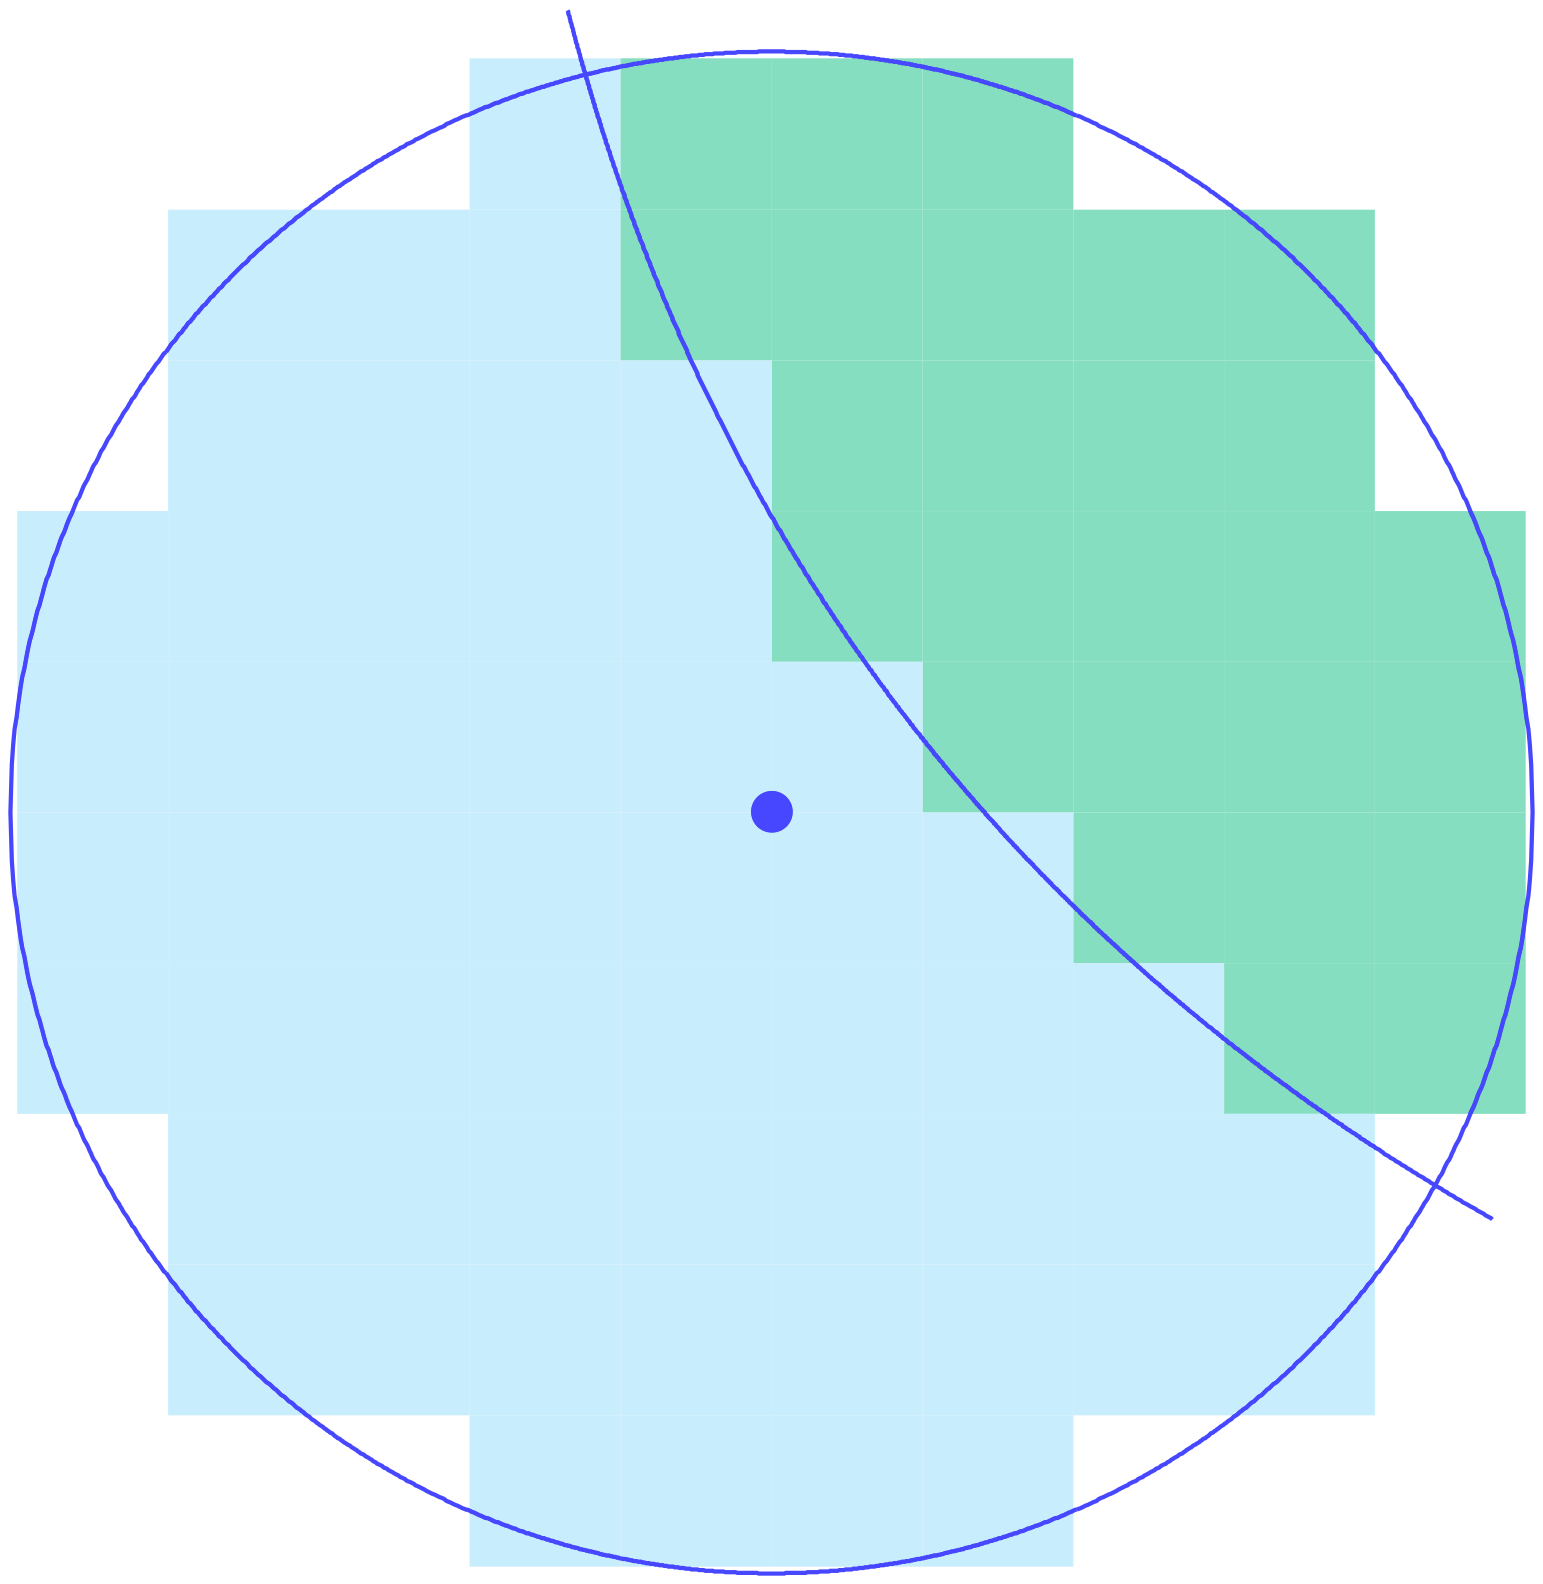
\includegraphics[scale=0.59]{media/2-shabaka/1-vor/dem2.png}
\label{fig:vor2}}
\subfigure[]{%
		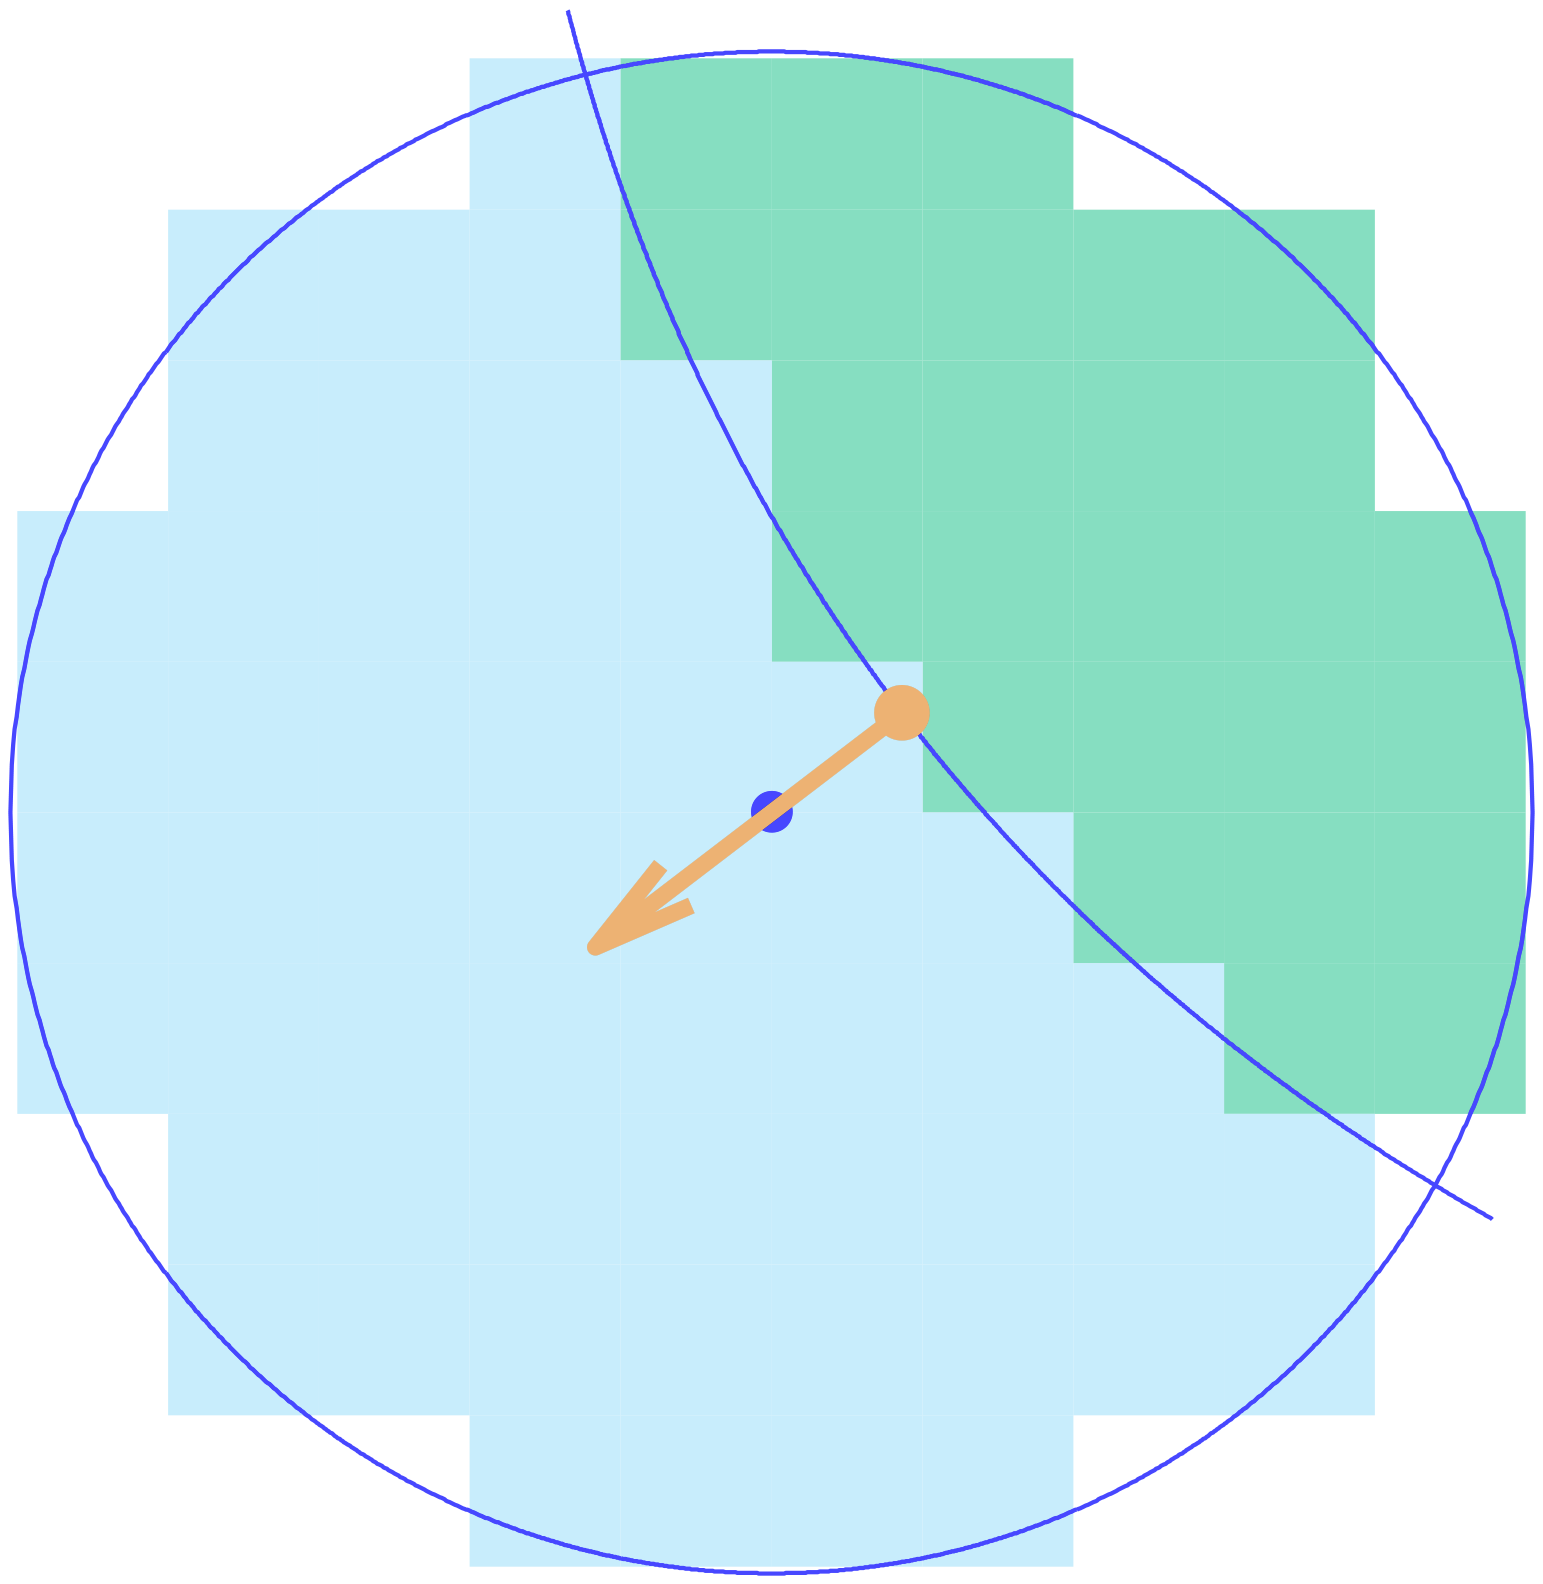
\includegraphics[scale=0.59]{media/2-shabaka/1-vor/dem3.png}
\label{fig:vor3}}
\subfigure[]{%
		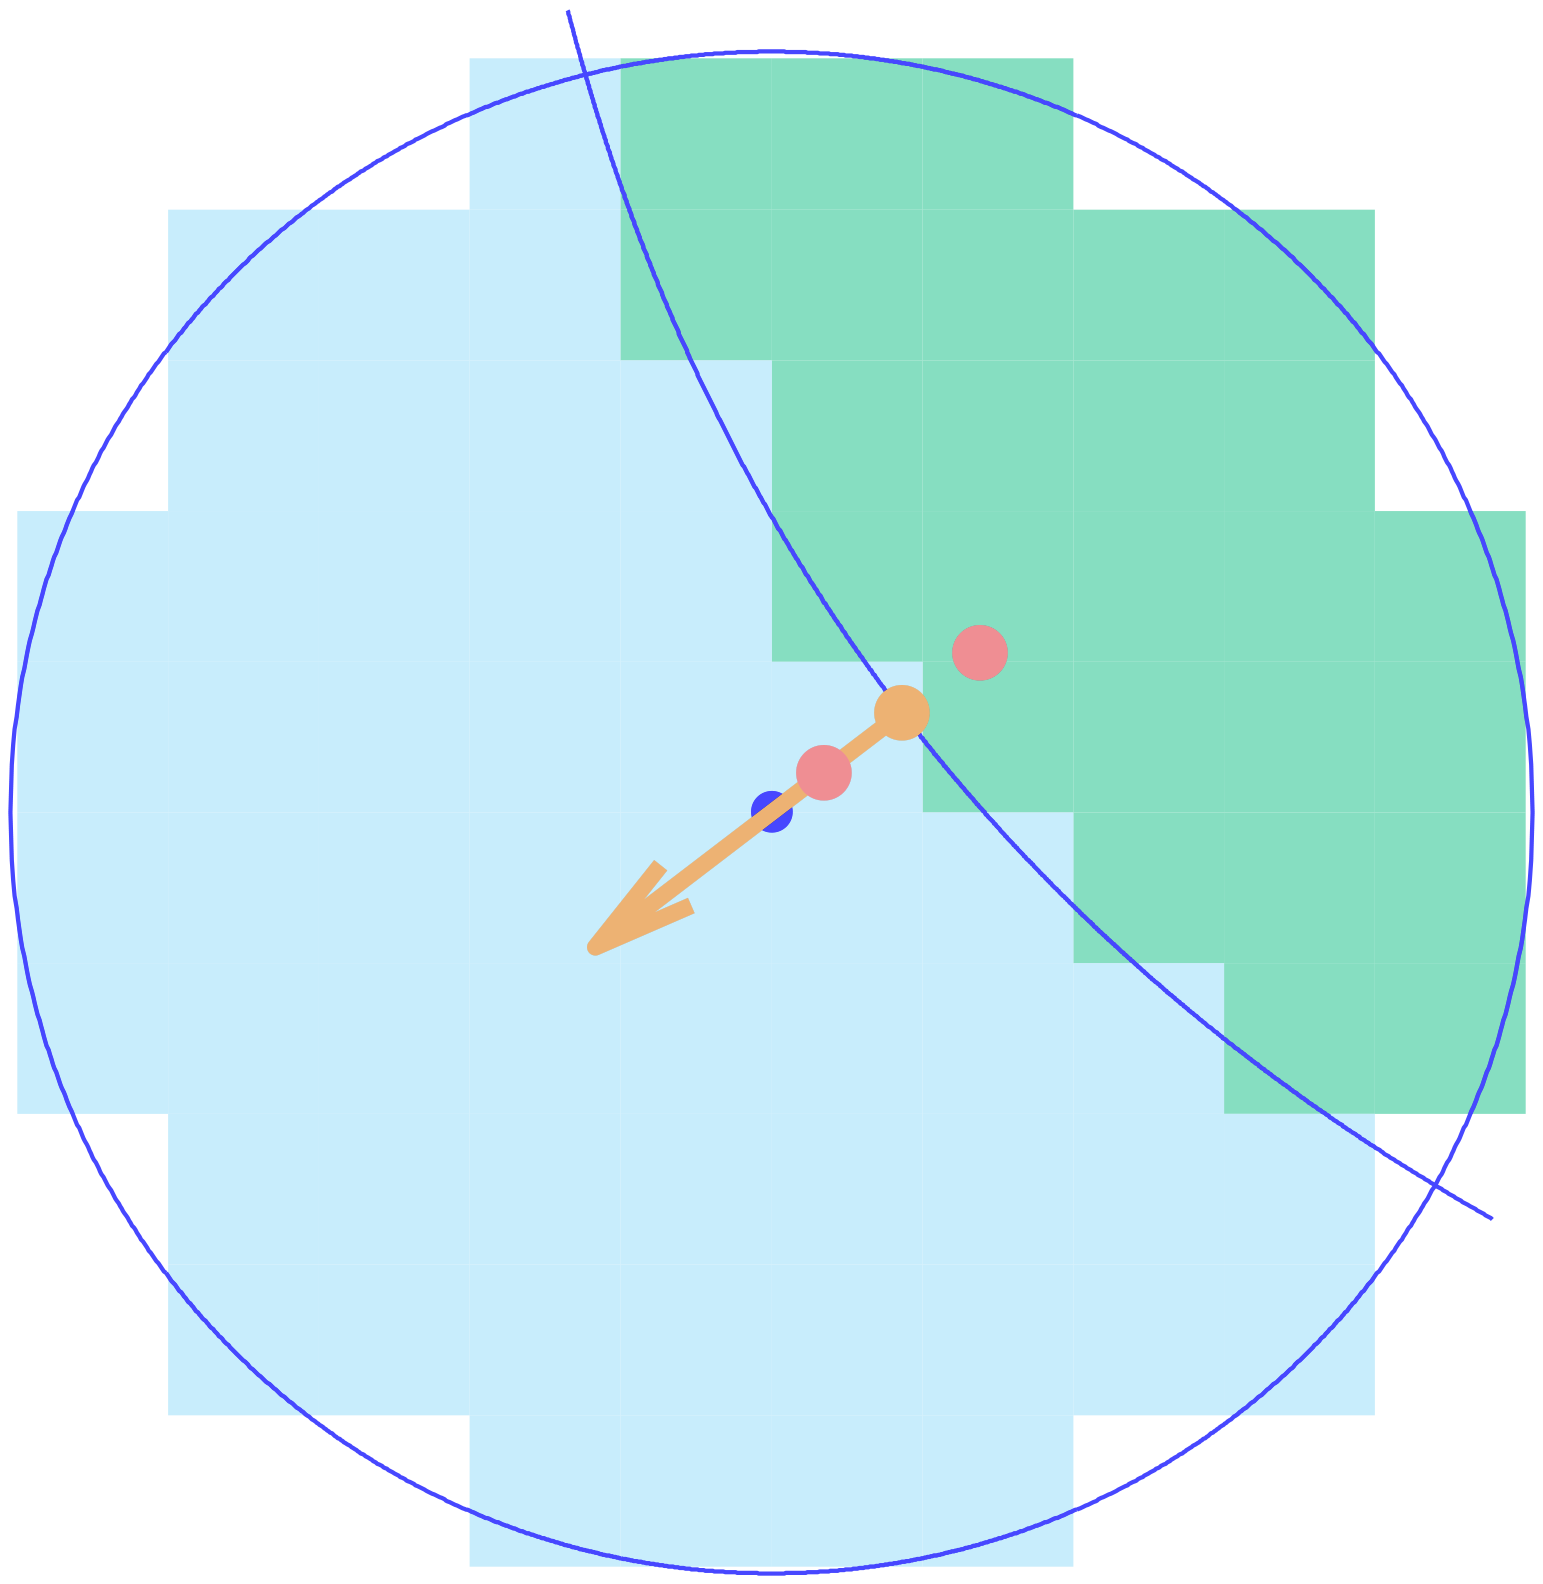
\includegraphics[scale=0.59]{media/2-shabaka/1-vor/dem4.png}
\label{fig:vor4}}
%
\caption{(a) Sample window of segmented image, (b) interface approximation, (c) point/normal placement, and d) Voronoi site placement}
\label{fig:vor}
\end{figure}

\begin{figure}[ht]
\centering
\subfigure[]{%
		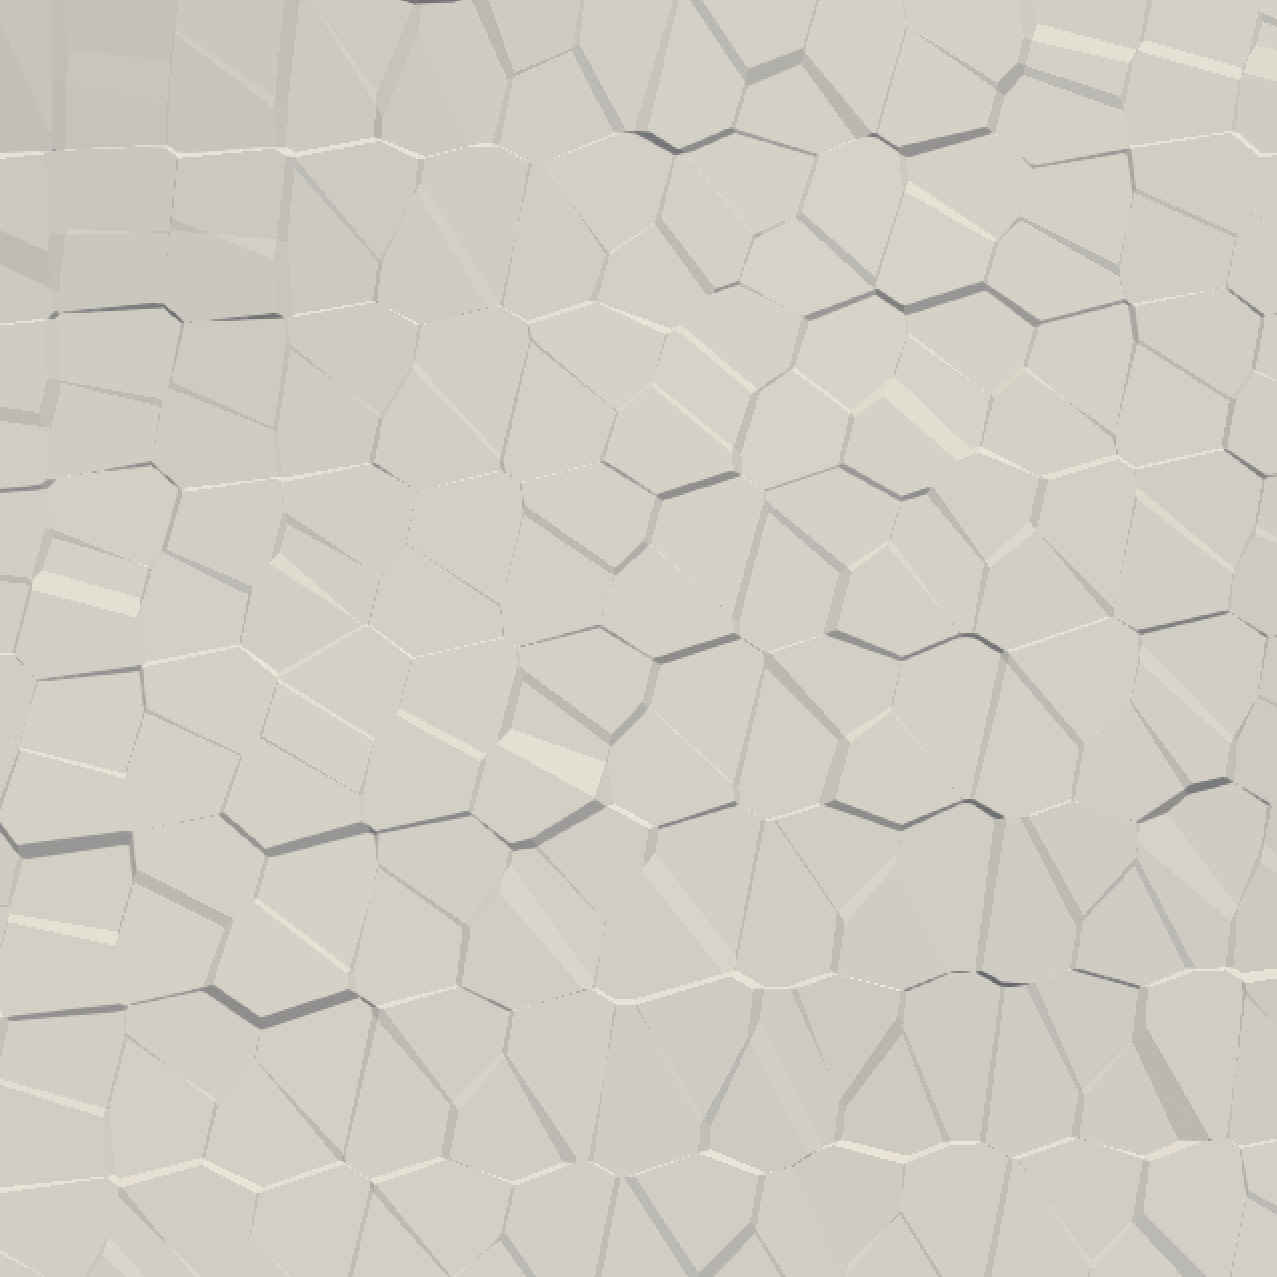
\includegraphics[scale=0.085]{media/2-shabaka/3-clean-zoom/1-init-zoom.png}
\label{fig:cross1-1}}		
\subfigure[]{%
		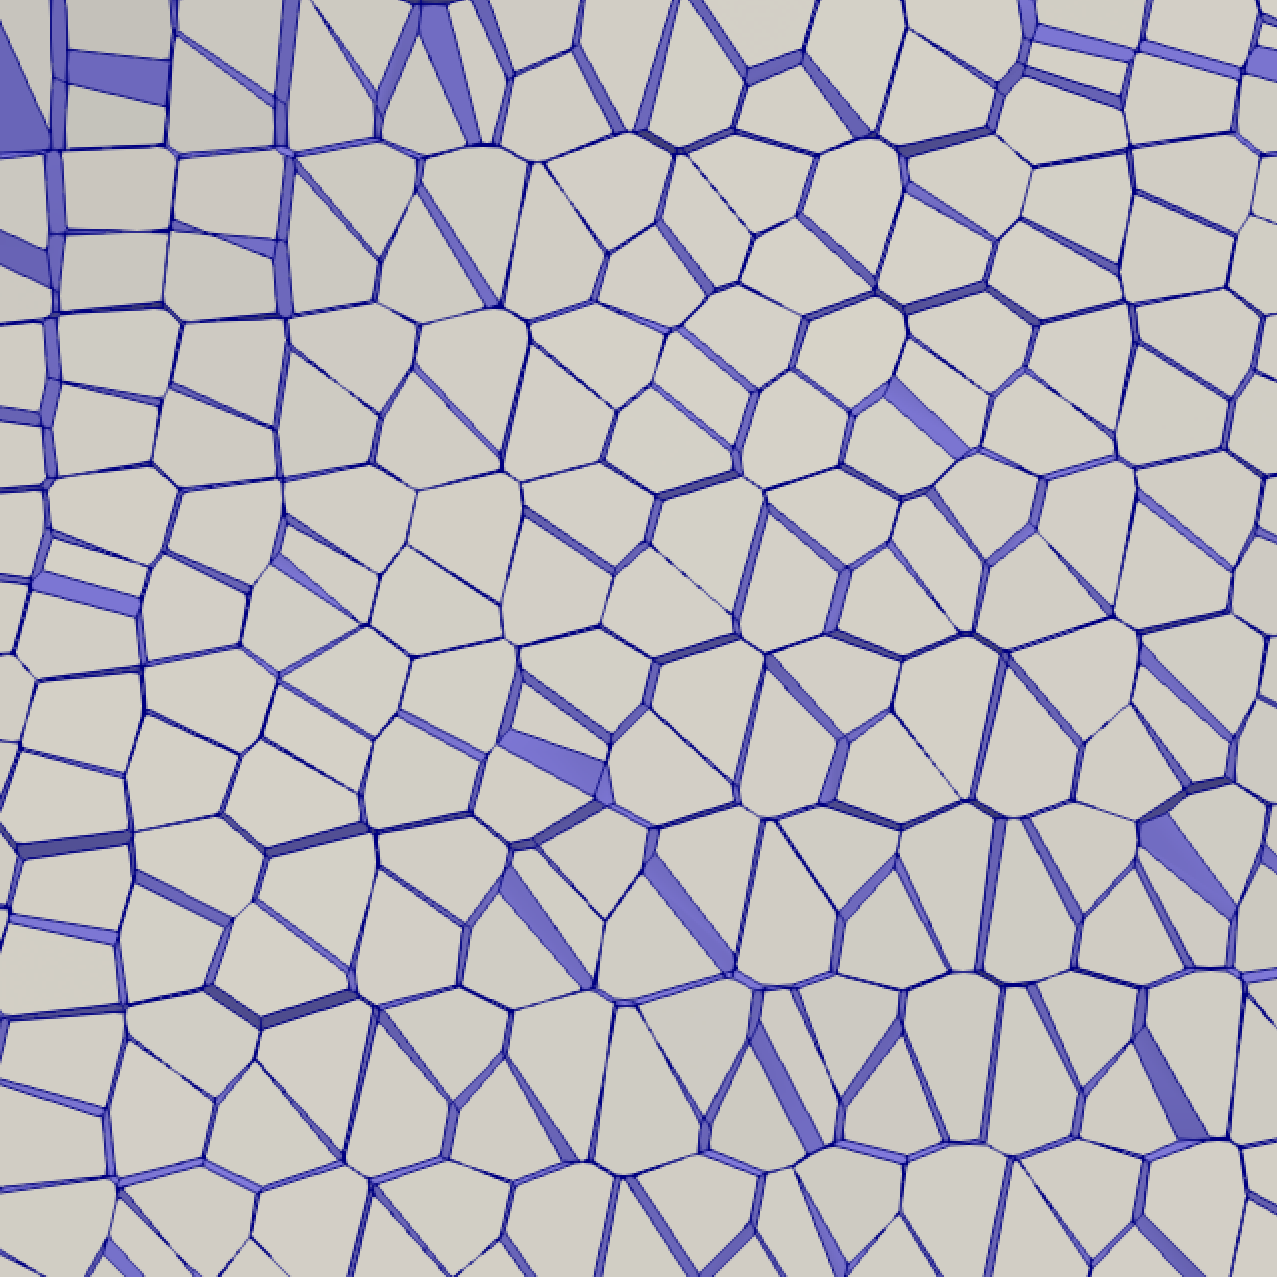
\includegraphics[scale=0.085]{media/2-shabaka/3-clean-zoom/2-badfacets-zoom.png}
\label{fig:cross1-2}}		
\subfigure[]{%
		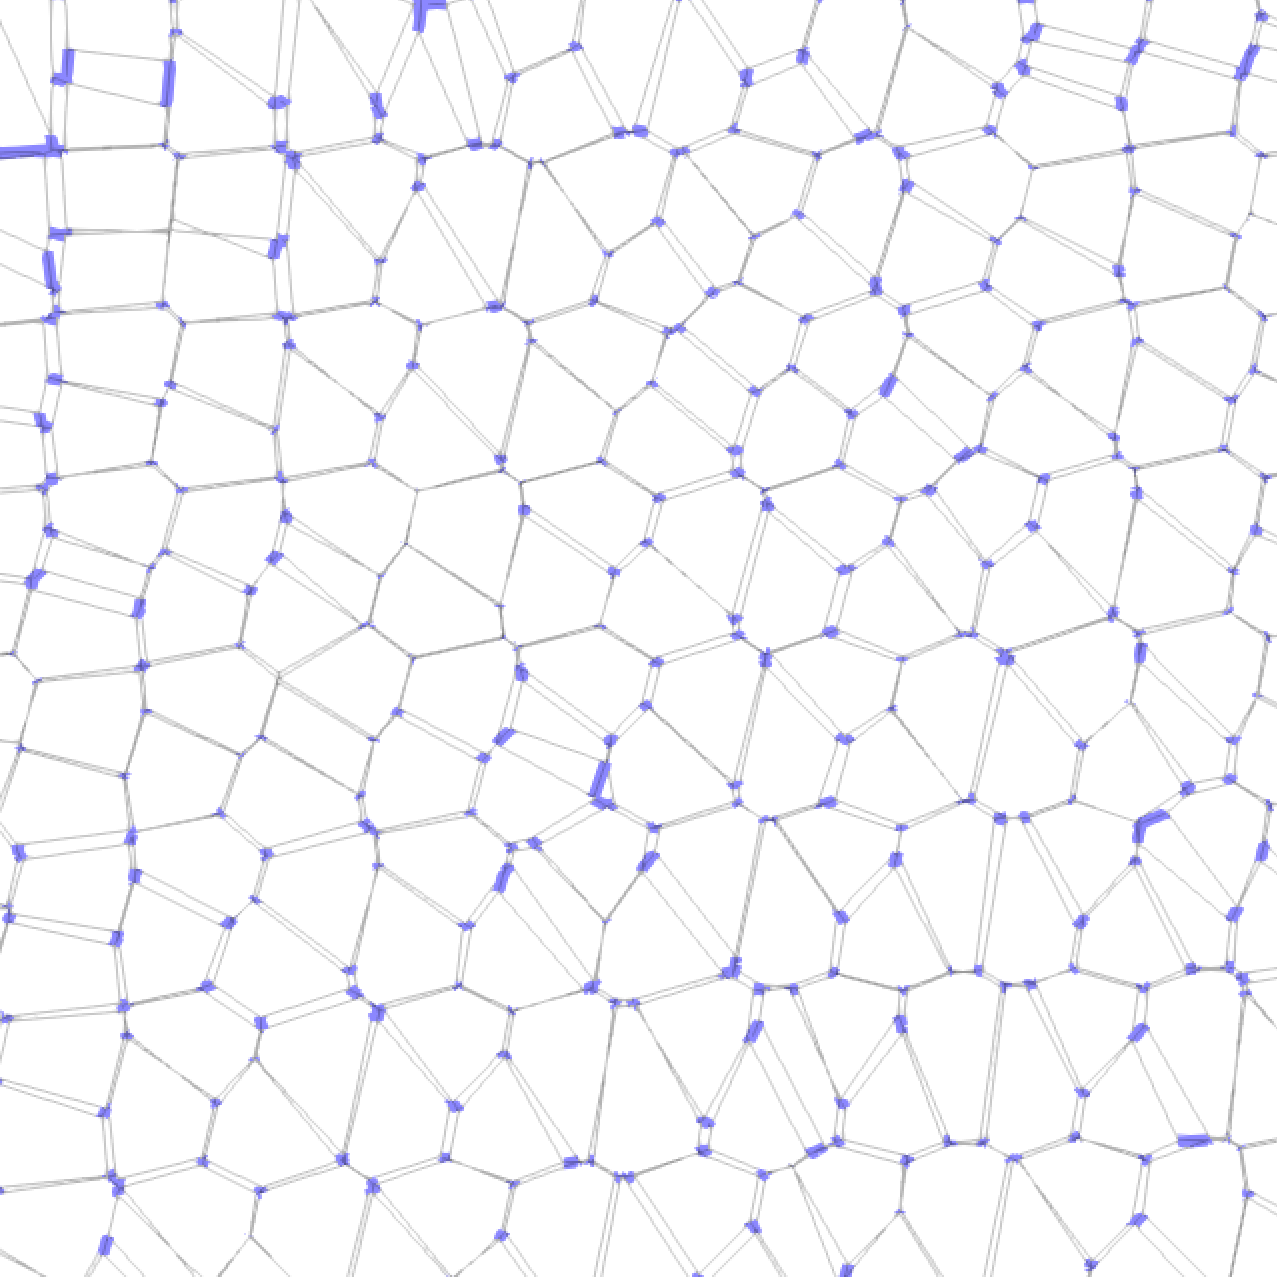
\includegraphics[scale=0.085]{media/2-shabaka/3-clean-zoom/3-badsegs-zoom.png}		
\label{fig:cross1-3}}					
\subfigure[]{%
		
\includegraphics[scale=0.085]{media/2-shabaka/3-clean-zoom/4-fine-zoom.png}
\label{fig:cross1-4}}				
%
\caption{Clean-up of undesirable ``cross-talk'' facets for a surface patch: (a) initial surface following Voronoi-based surface reconstruction, (b) identification of ``cross-talk'' facets, (c) identification of edges to be collapsed, (d) final cleaned surface.}
\label{fig:cross1}
\end{figure}

\begin{figure}[ht]
\centering
\subfigure[]{%
		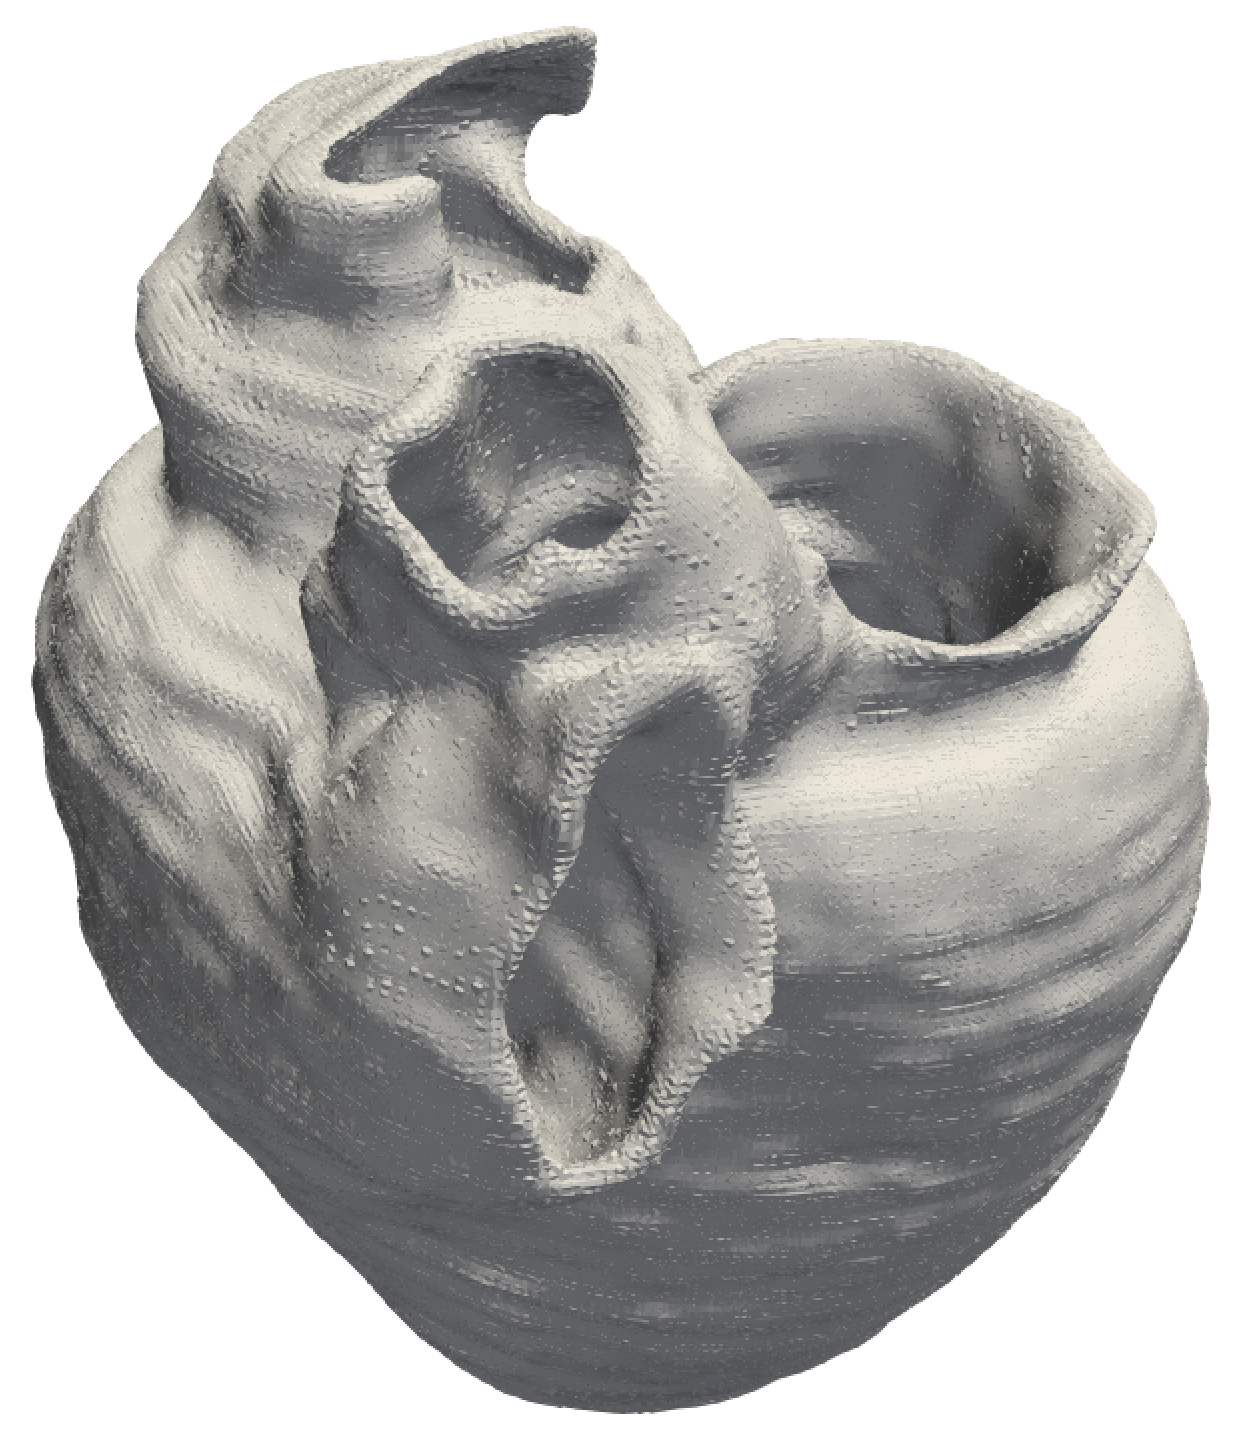
\includegraphics[scale=0.075]{media/2-shabaka/4-clean/1-init.png}
\label{fig:cross2-1}}		
\subfigure[]{%
		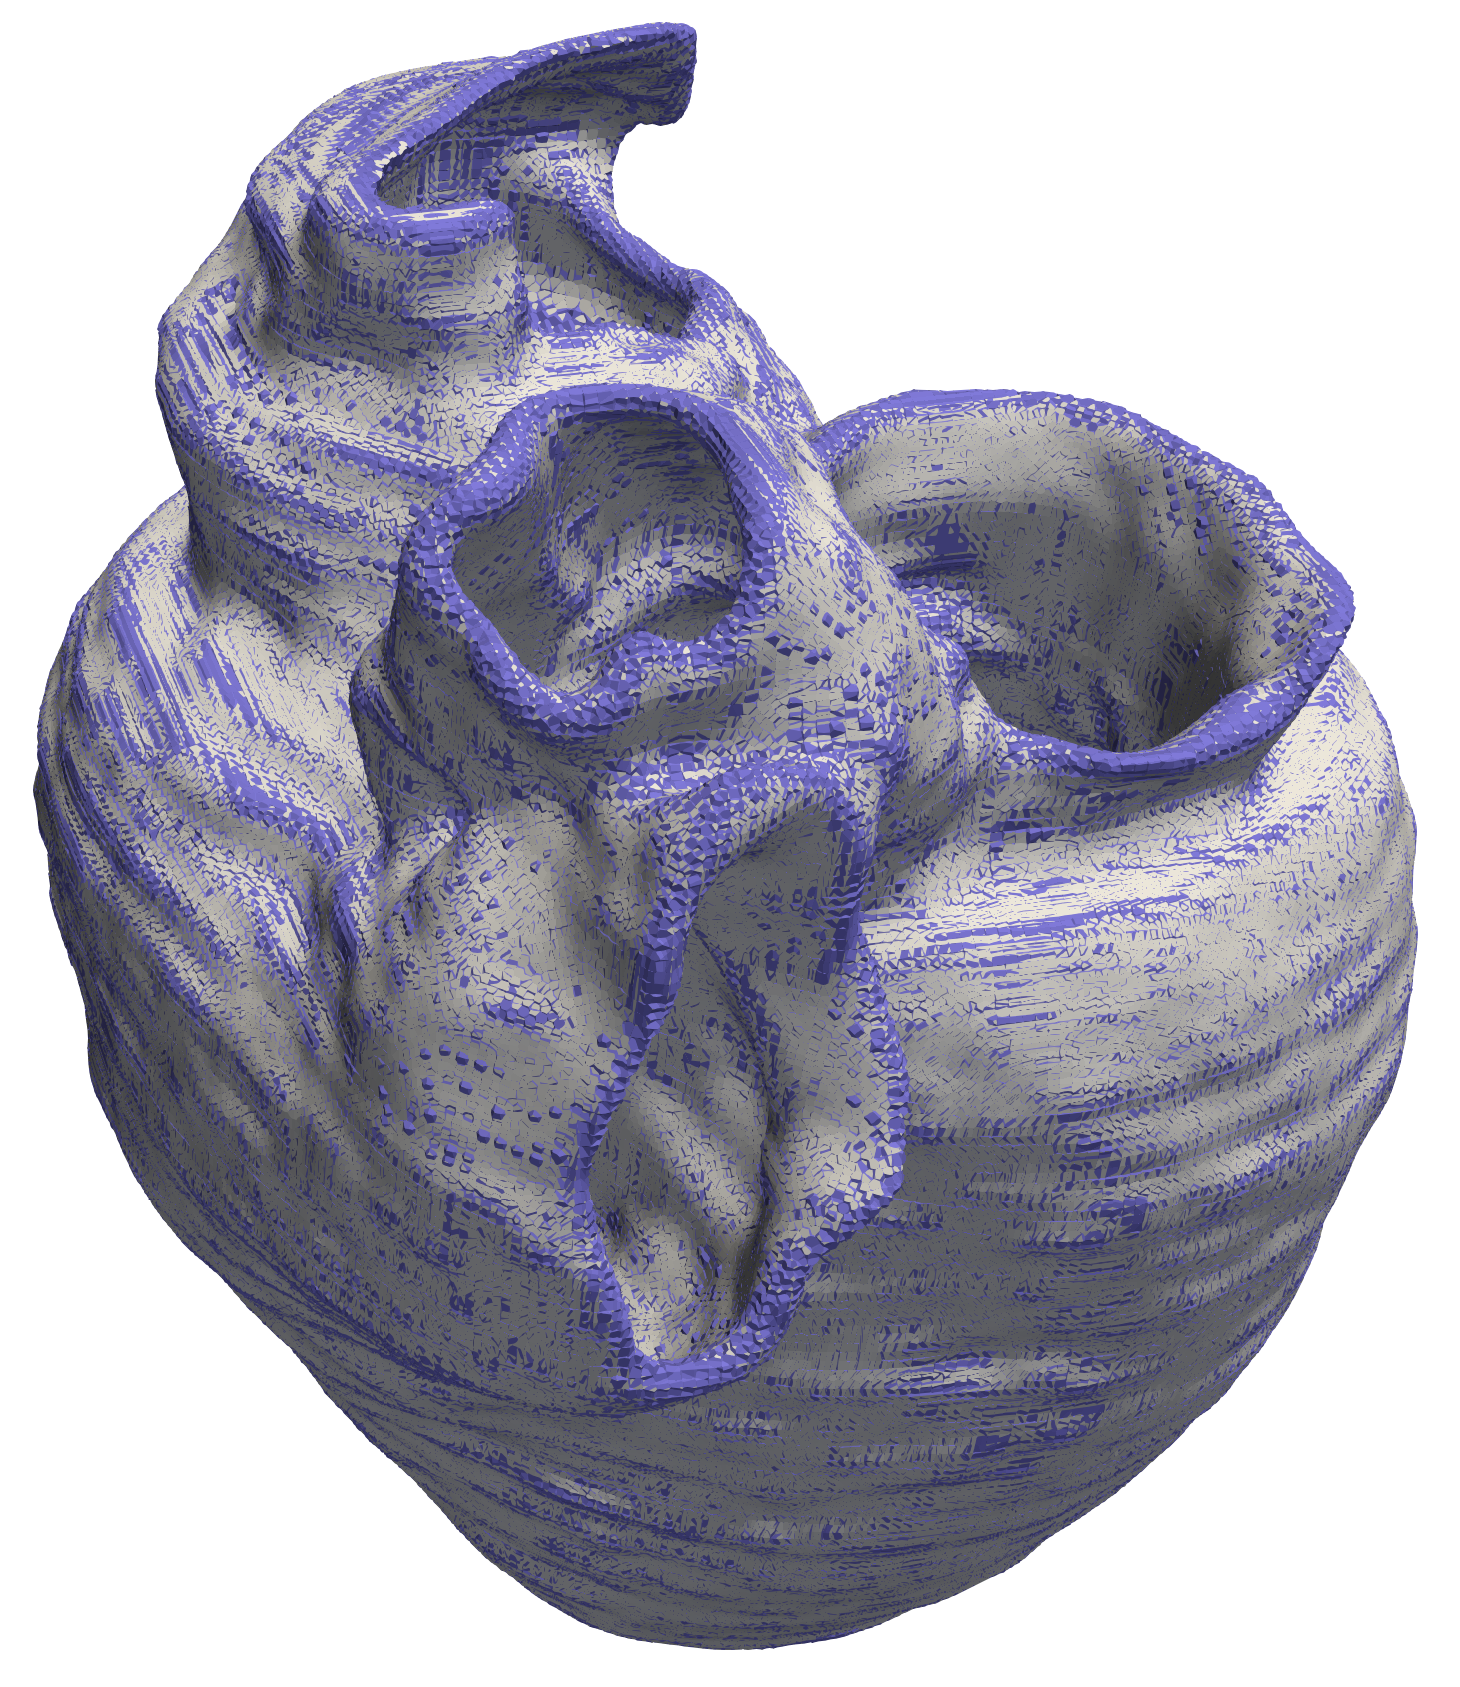
\includegraphics[scale=0.075]{media/2-shabaka/4-clean/2-badfacets.png}
\label{fig:cross2-2}}		
\subfigure[]{%
		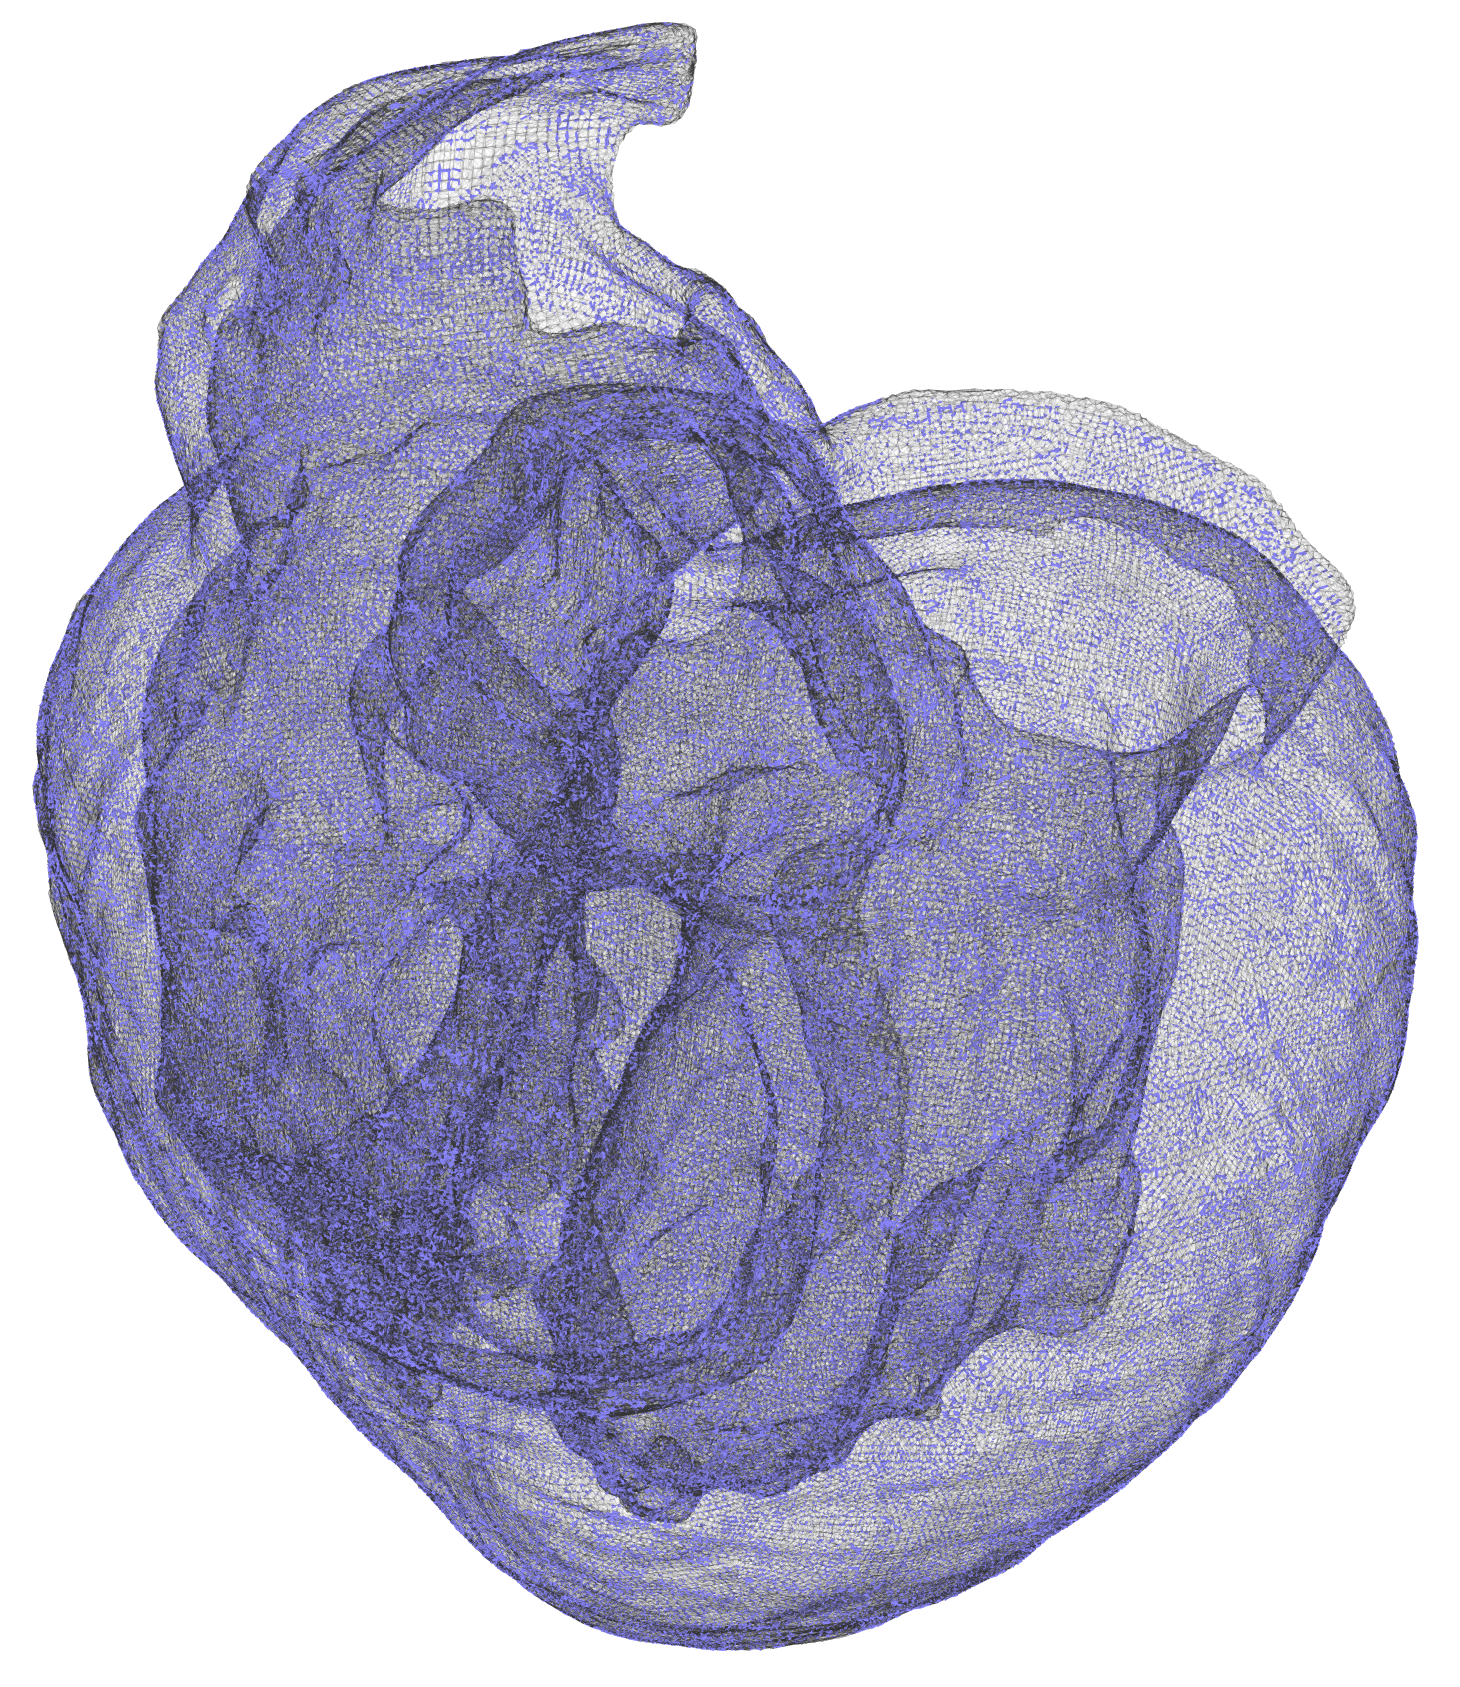
\includegraphics[scale=0.075]{media/2-shabaka/4-clean/3-badsegs.png}	
\label{fig:cross2-3}}						
\subfigure[]{%
		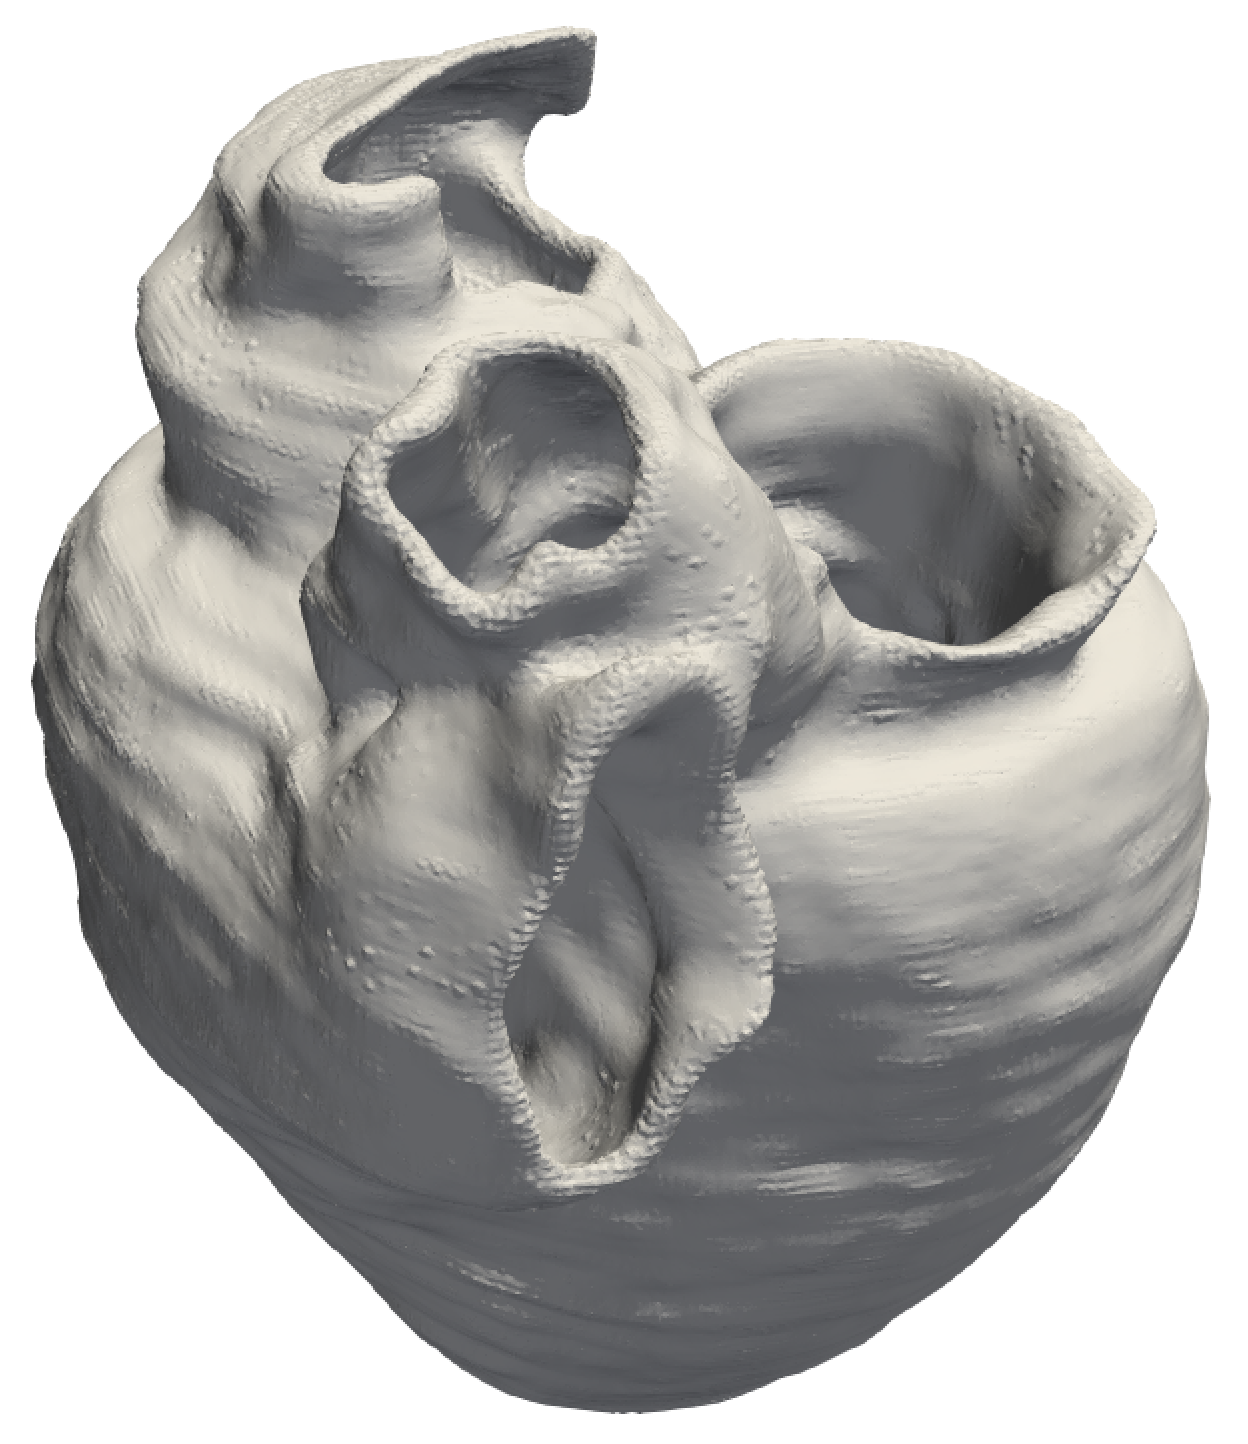
\includegraphics[scale=0.075]{media/2-shabaka/4-clean/4-fine.png}		
\label{fig:cross2-4}}		
%
\caption{Clean-up of undesirable ``cross-talk'' facets for surface of \textit{ex-vivo} human heart: (a) initial surface following Voronoi-based surface reconstruction, (b) identification of ``cross-talk'' facets, (c) identification of edges to be collapsed, (d) final cleaned surface.}
\label{fig:cross2}
\end{figure}

\begin{figure}[ht!]
\centering
\subfigure[]{%
		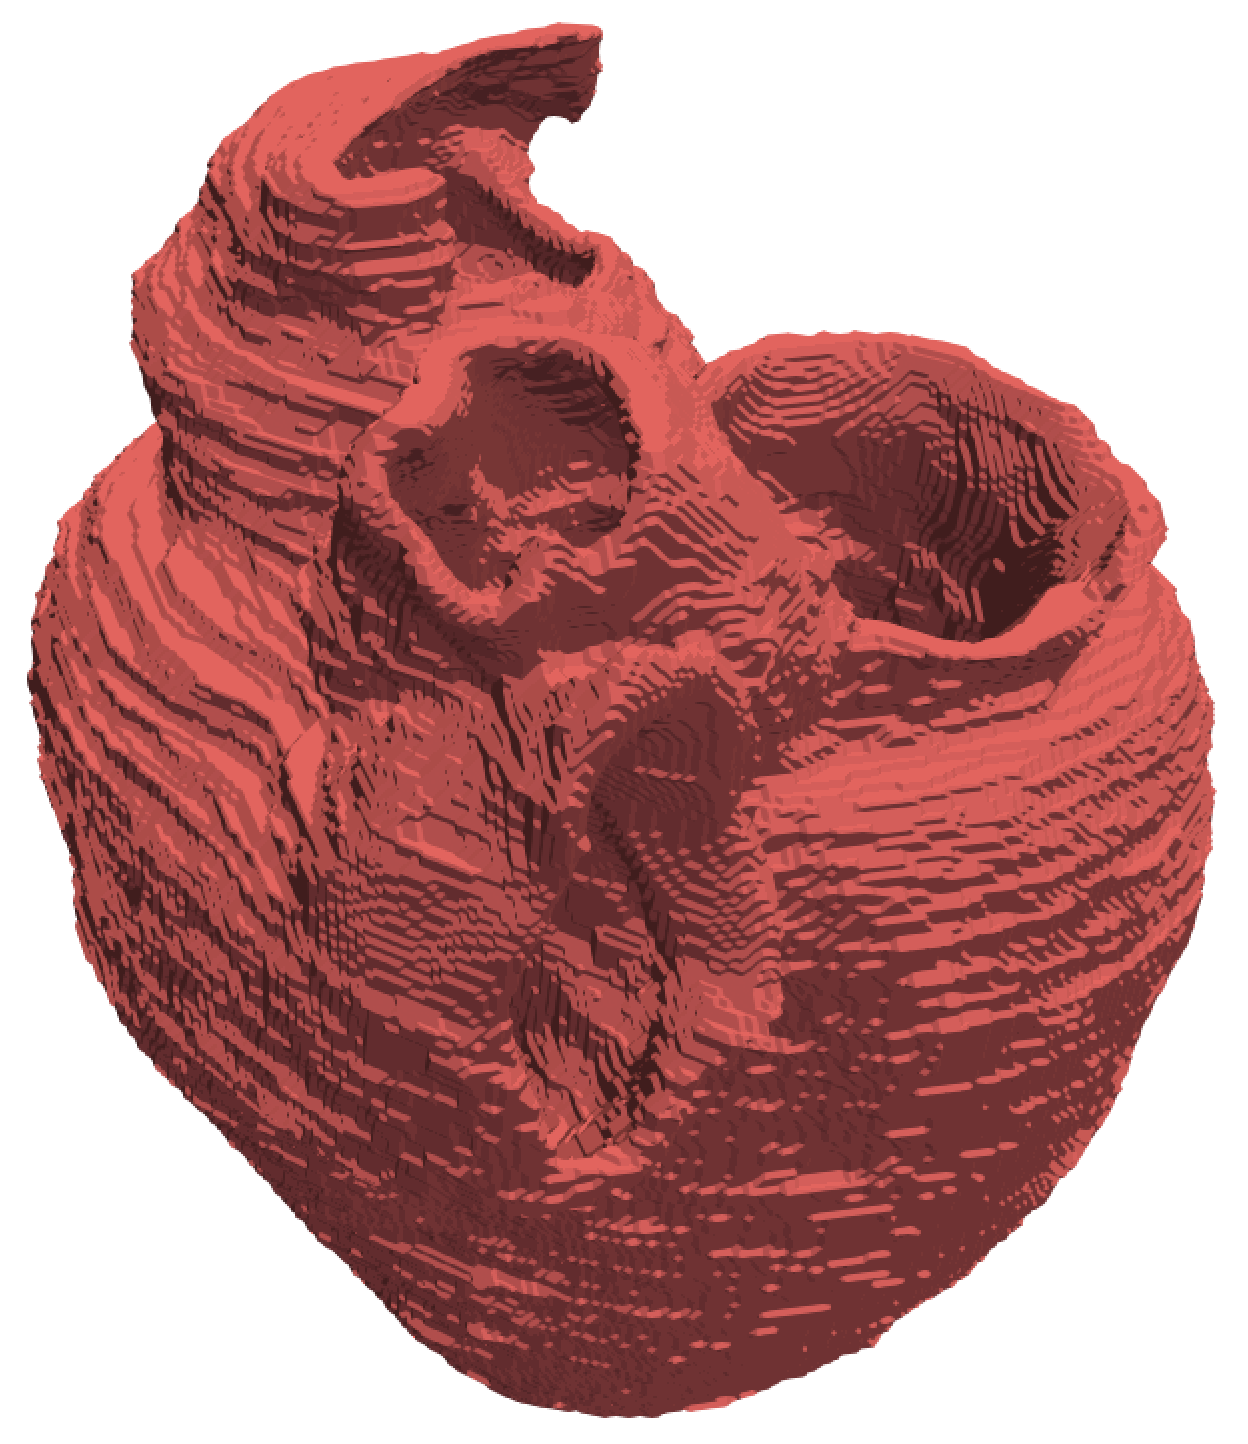
\includegraphics[scale=0.1]{media/2-shabaka/2-surf/1-seg.png}
\label{fig:shabakaseq1}}
\subfigure[]{%
		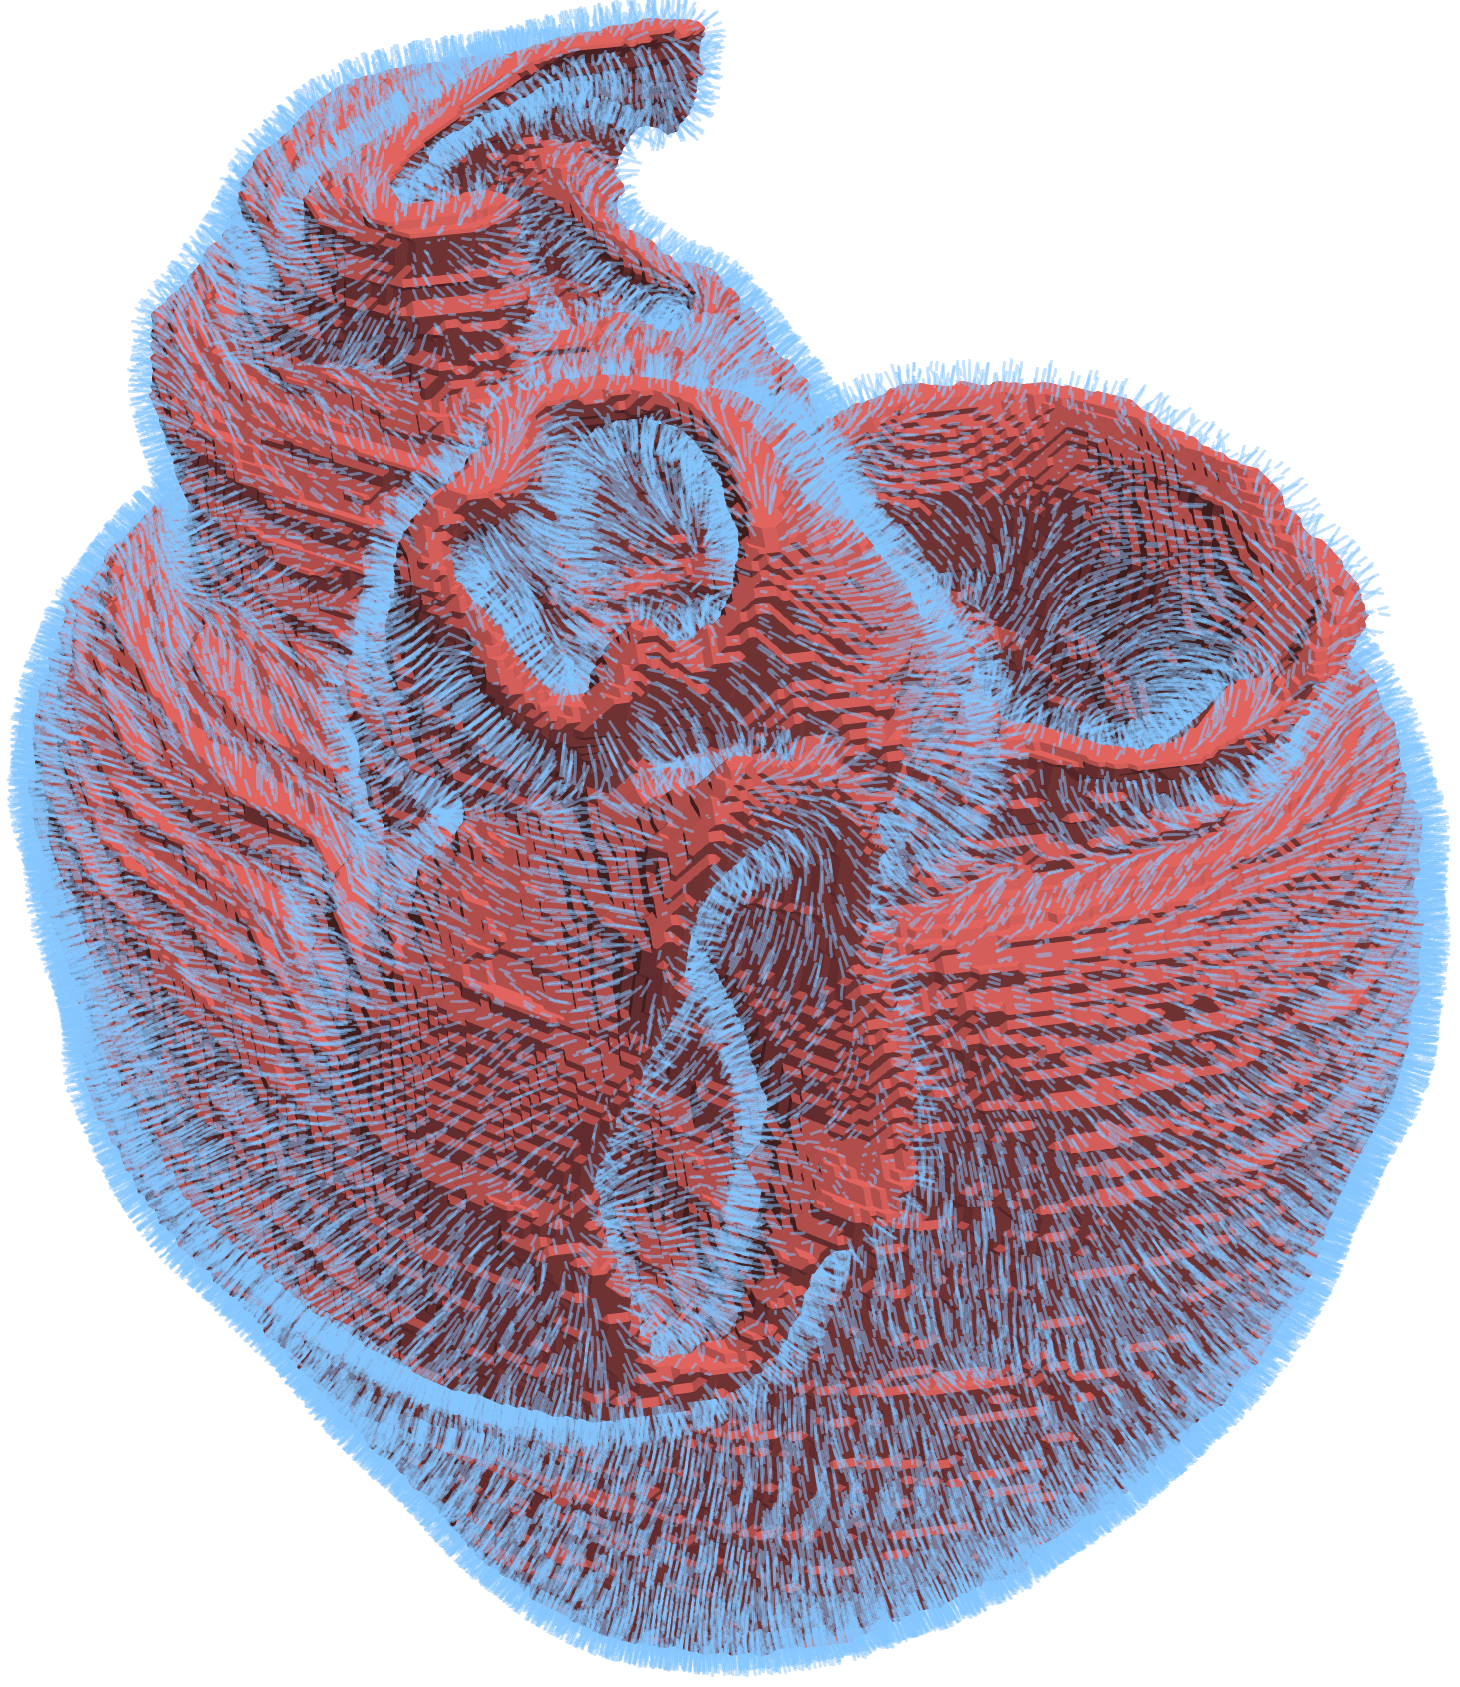
\includegraphics[scale=0.1]{media/2-shabaka/2-surf/2-normals.png}
\label{fig:shabakaseq2}}
\subfigure[]{%
		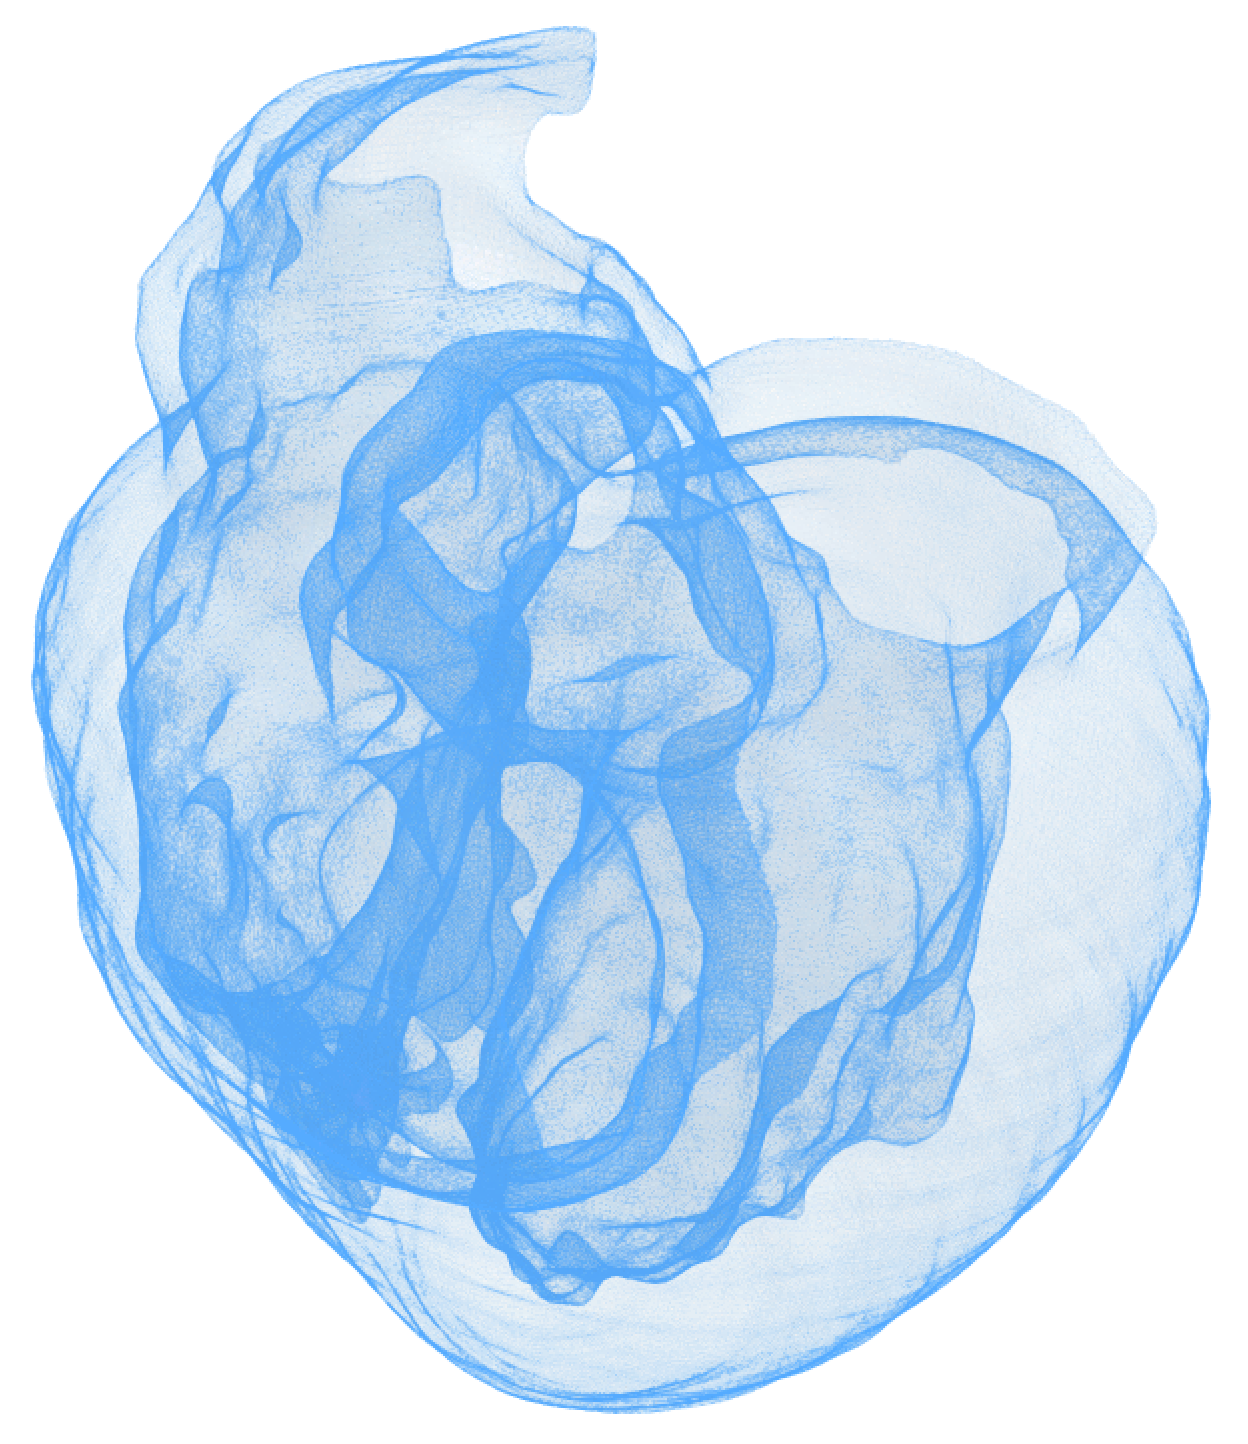
\includegraphics[scale=0.1]{media/2-shabaka/2-surf/3-ptcloud.png}
\label{fig:shabakaseq3}}
\subfigure[]{%
		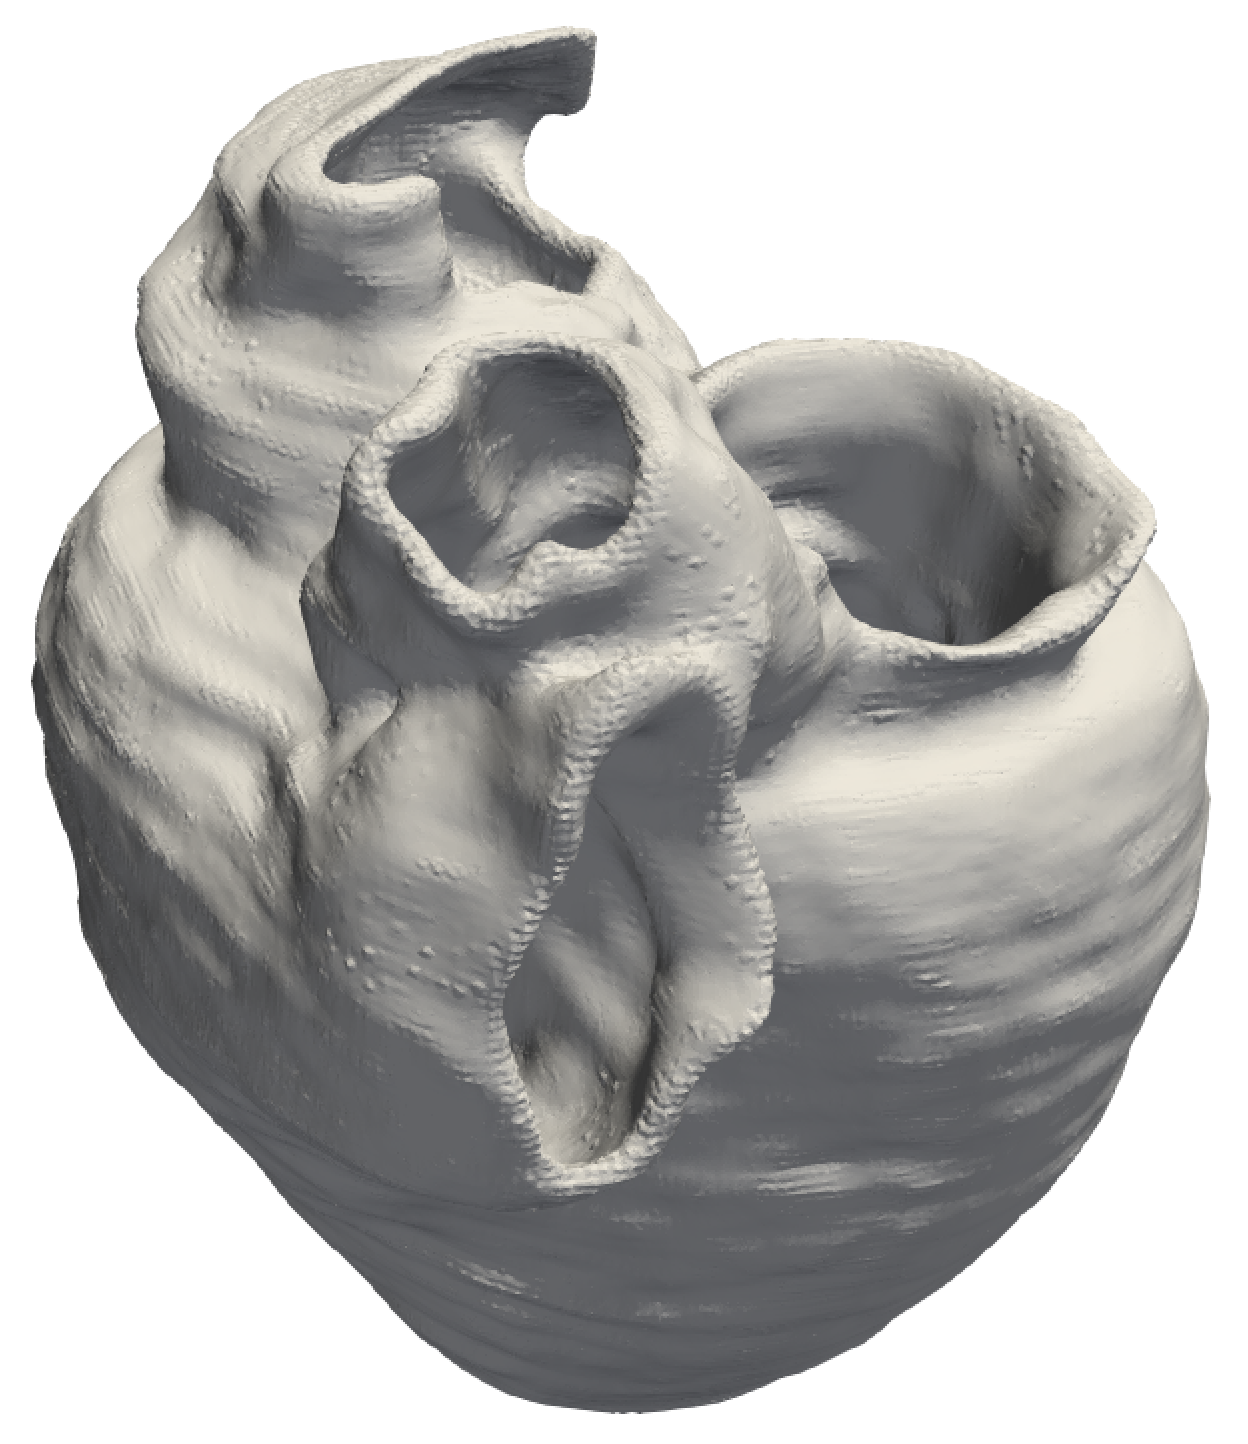
\includegraphics[scale=0.1]{media/2-shabaka/2-surf/4-finesurf.png}
\label{fig:shabakaseq4}}
\subfigure[]{%
		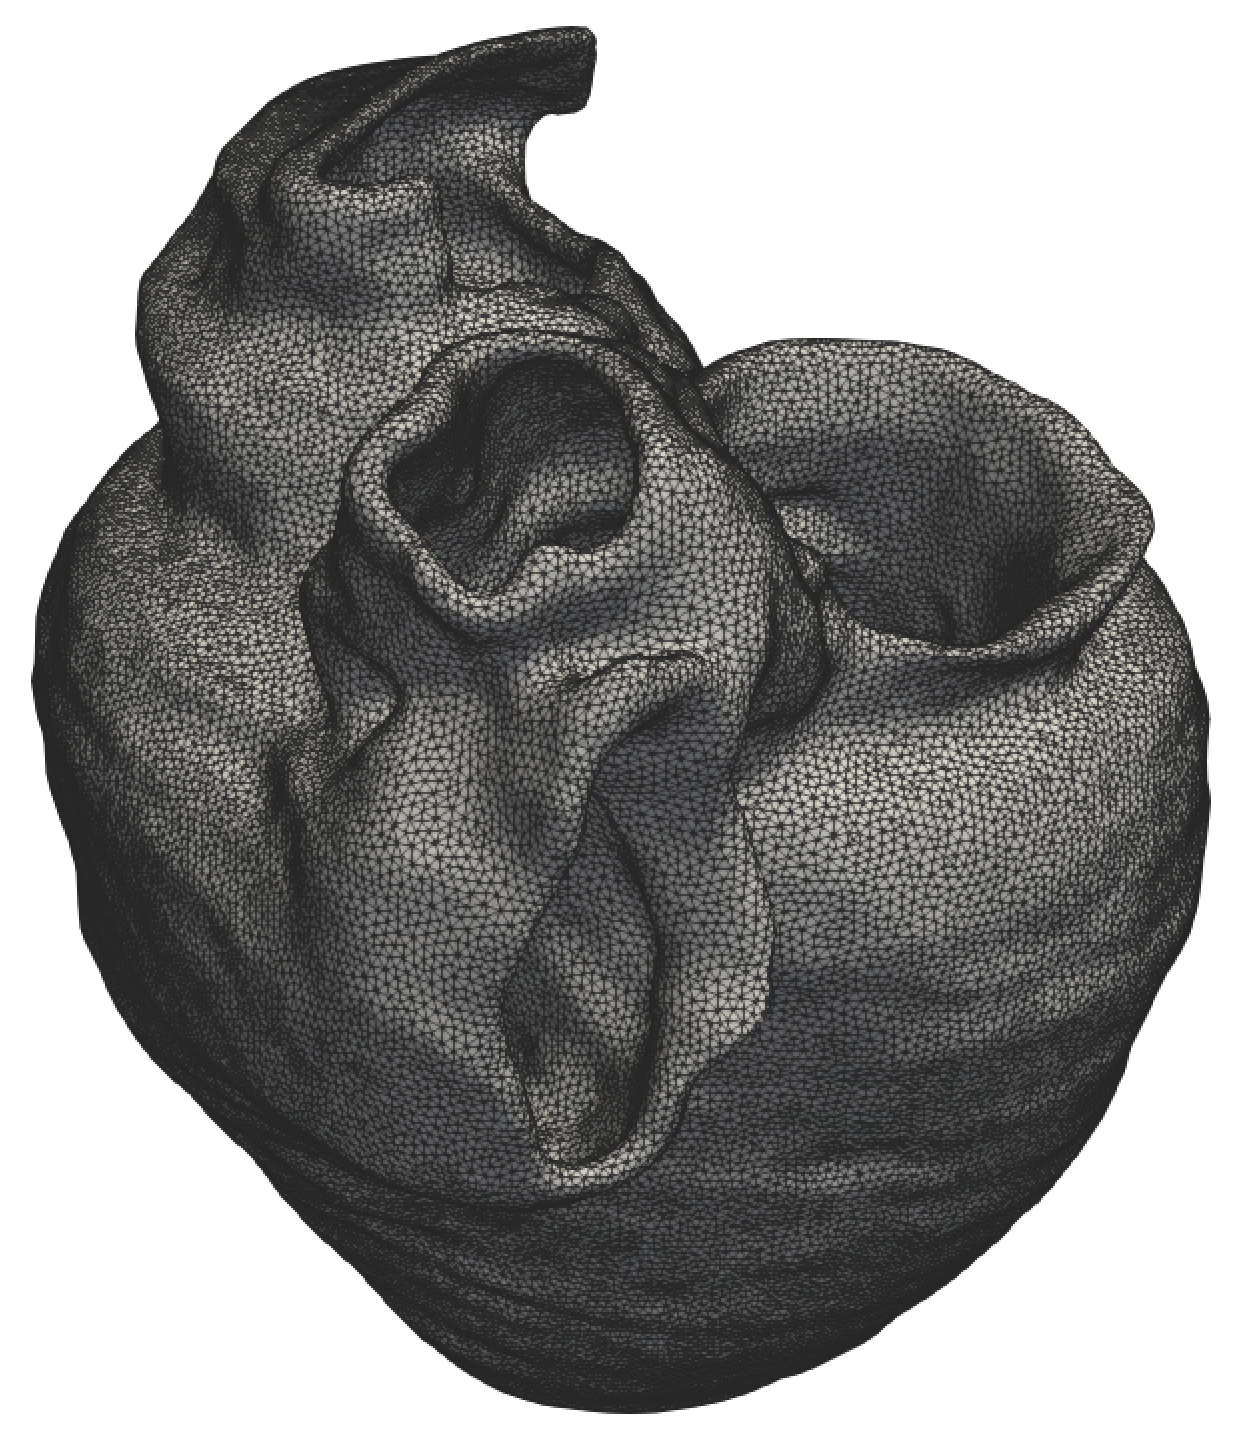
\includegraphics[scale=0.1]{media/2-shabaka/2-surf/5-surf.png}
\label{fig:shabakaseq5}}
%
\caption{(a) Segmented image, (b) point/normal placement, (c) oriented point cloud (normals not shown), c) cleaned surface mesh generated from Voronoi partition (edges not shown), and d) final decimated surface}
\label{fig:shabakaseq}
\end{figure}

\begin{figure}[ht!]
\centering
\vspace{2.5mm}
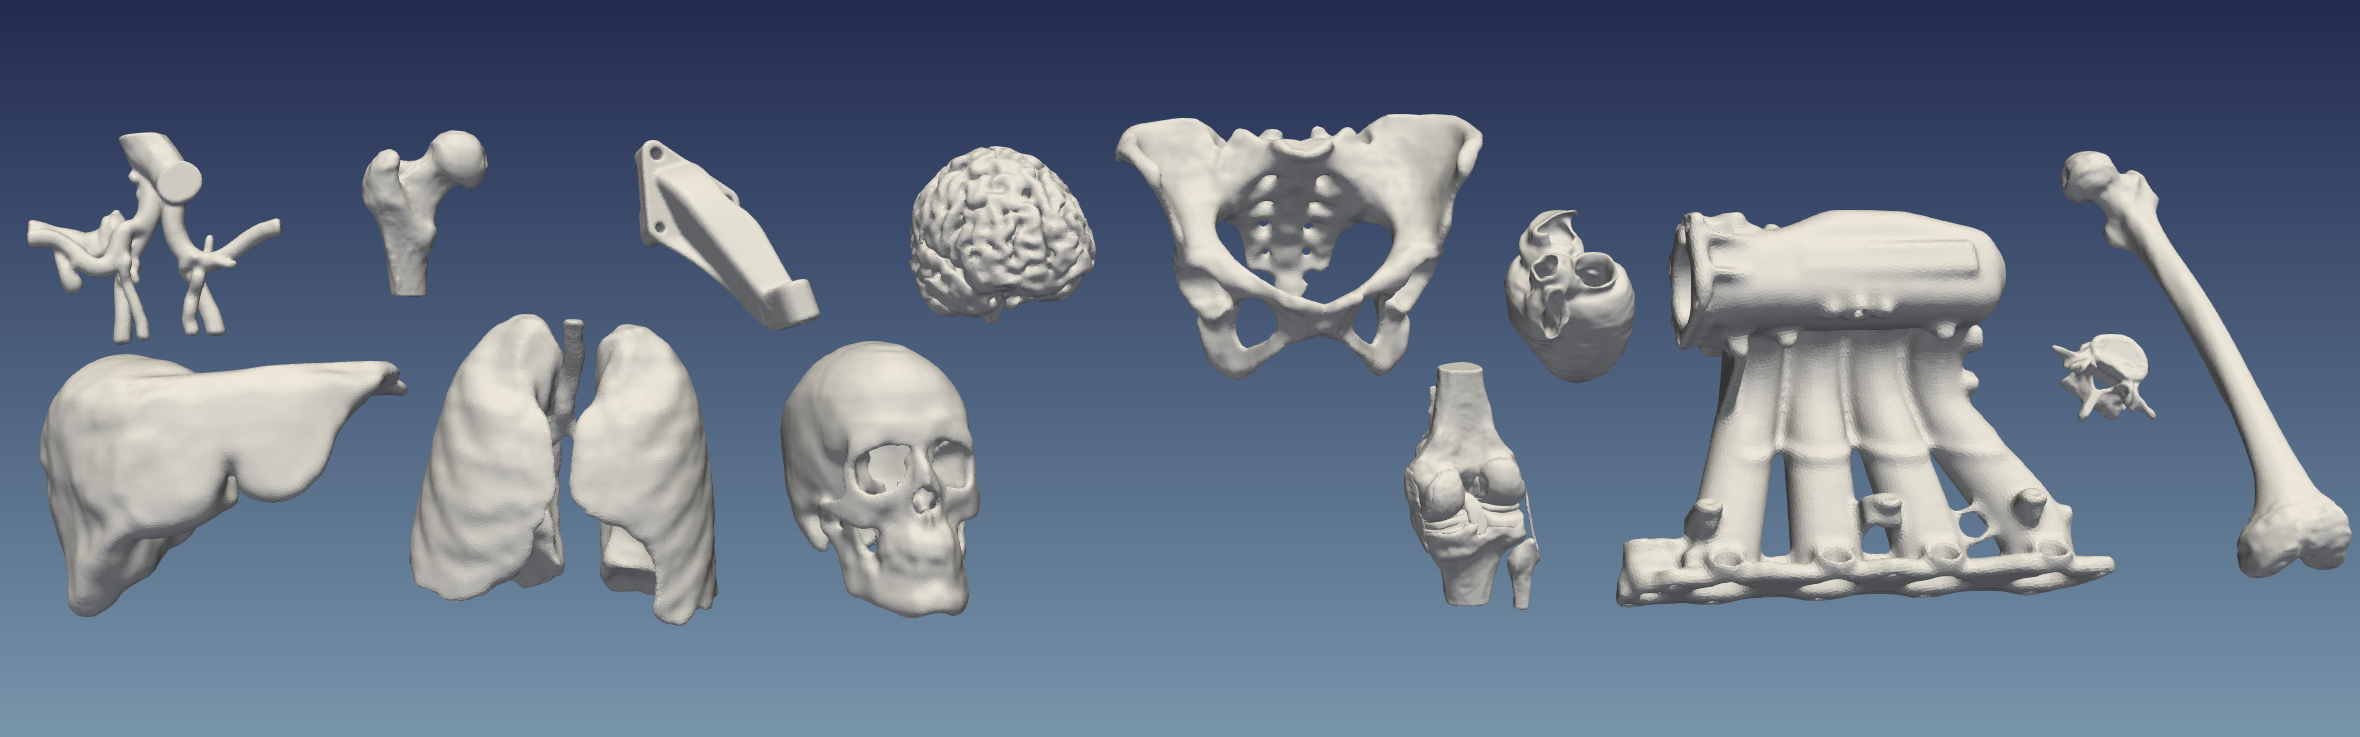
\includegraphics[width=1.0\textwidth]{media/2-shabaka/2-surf/6-showcase.png}
\caption{Suite of example surfaces generated from image data.}
\label{fig:showcase}
\end{figure}

\begin{figure}[ht!]
\centering
\vspace{2.5mm}
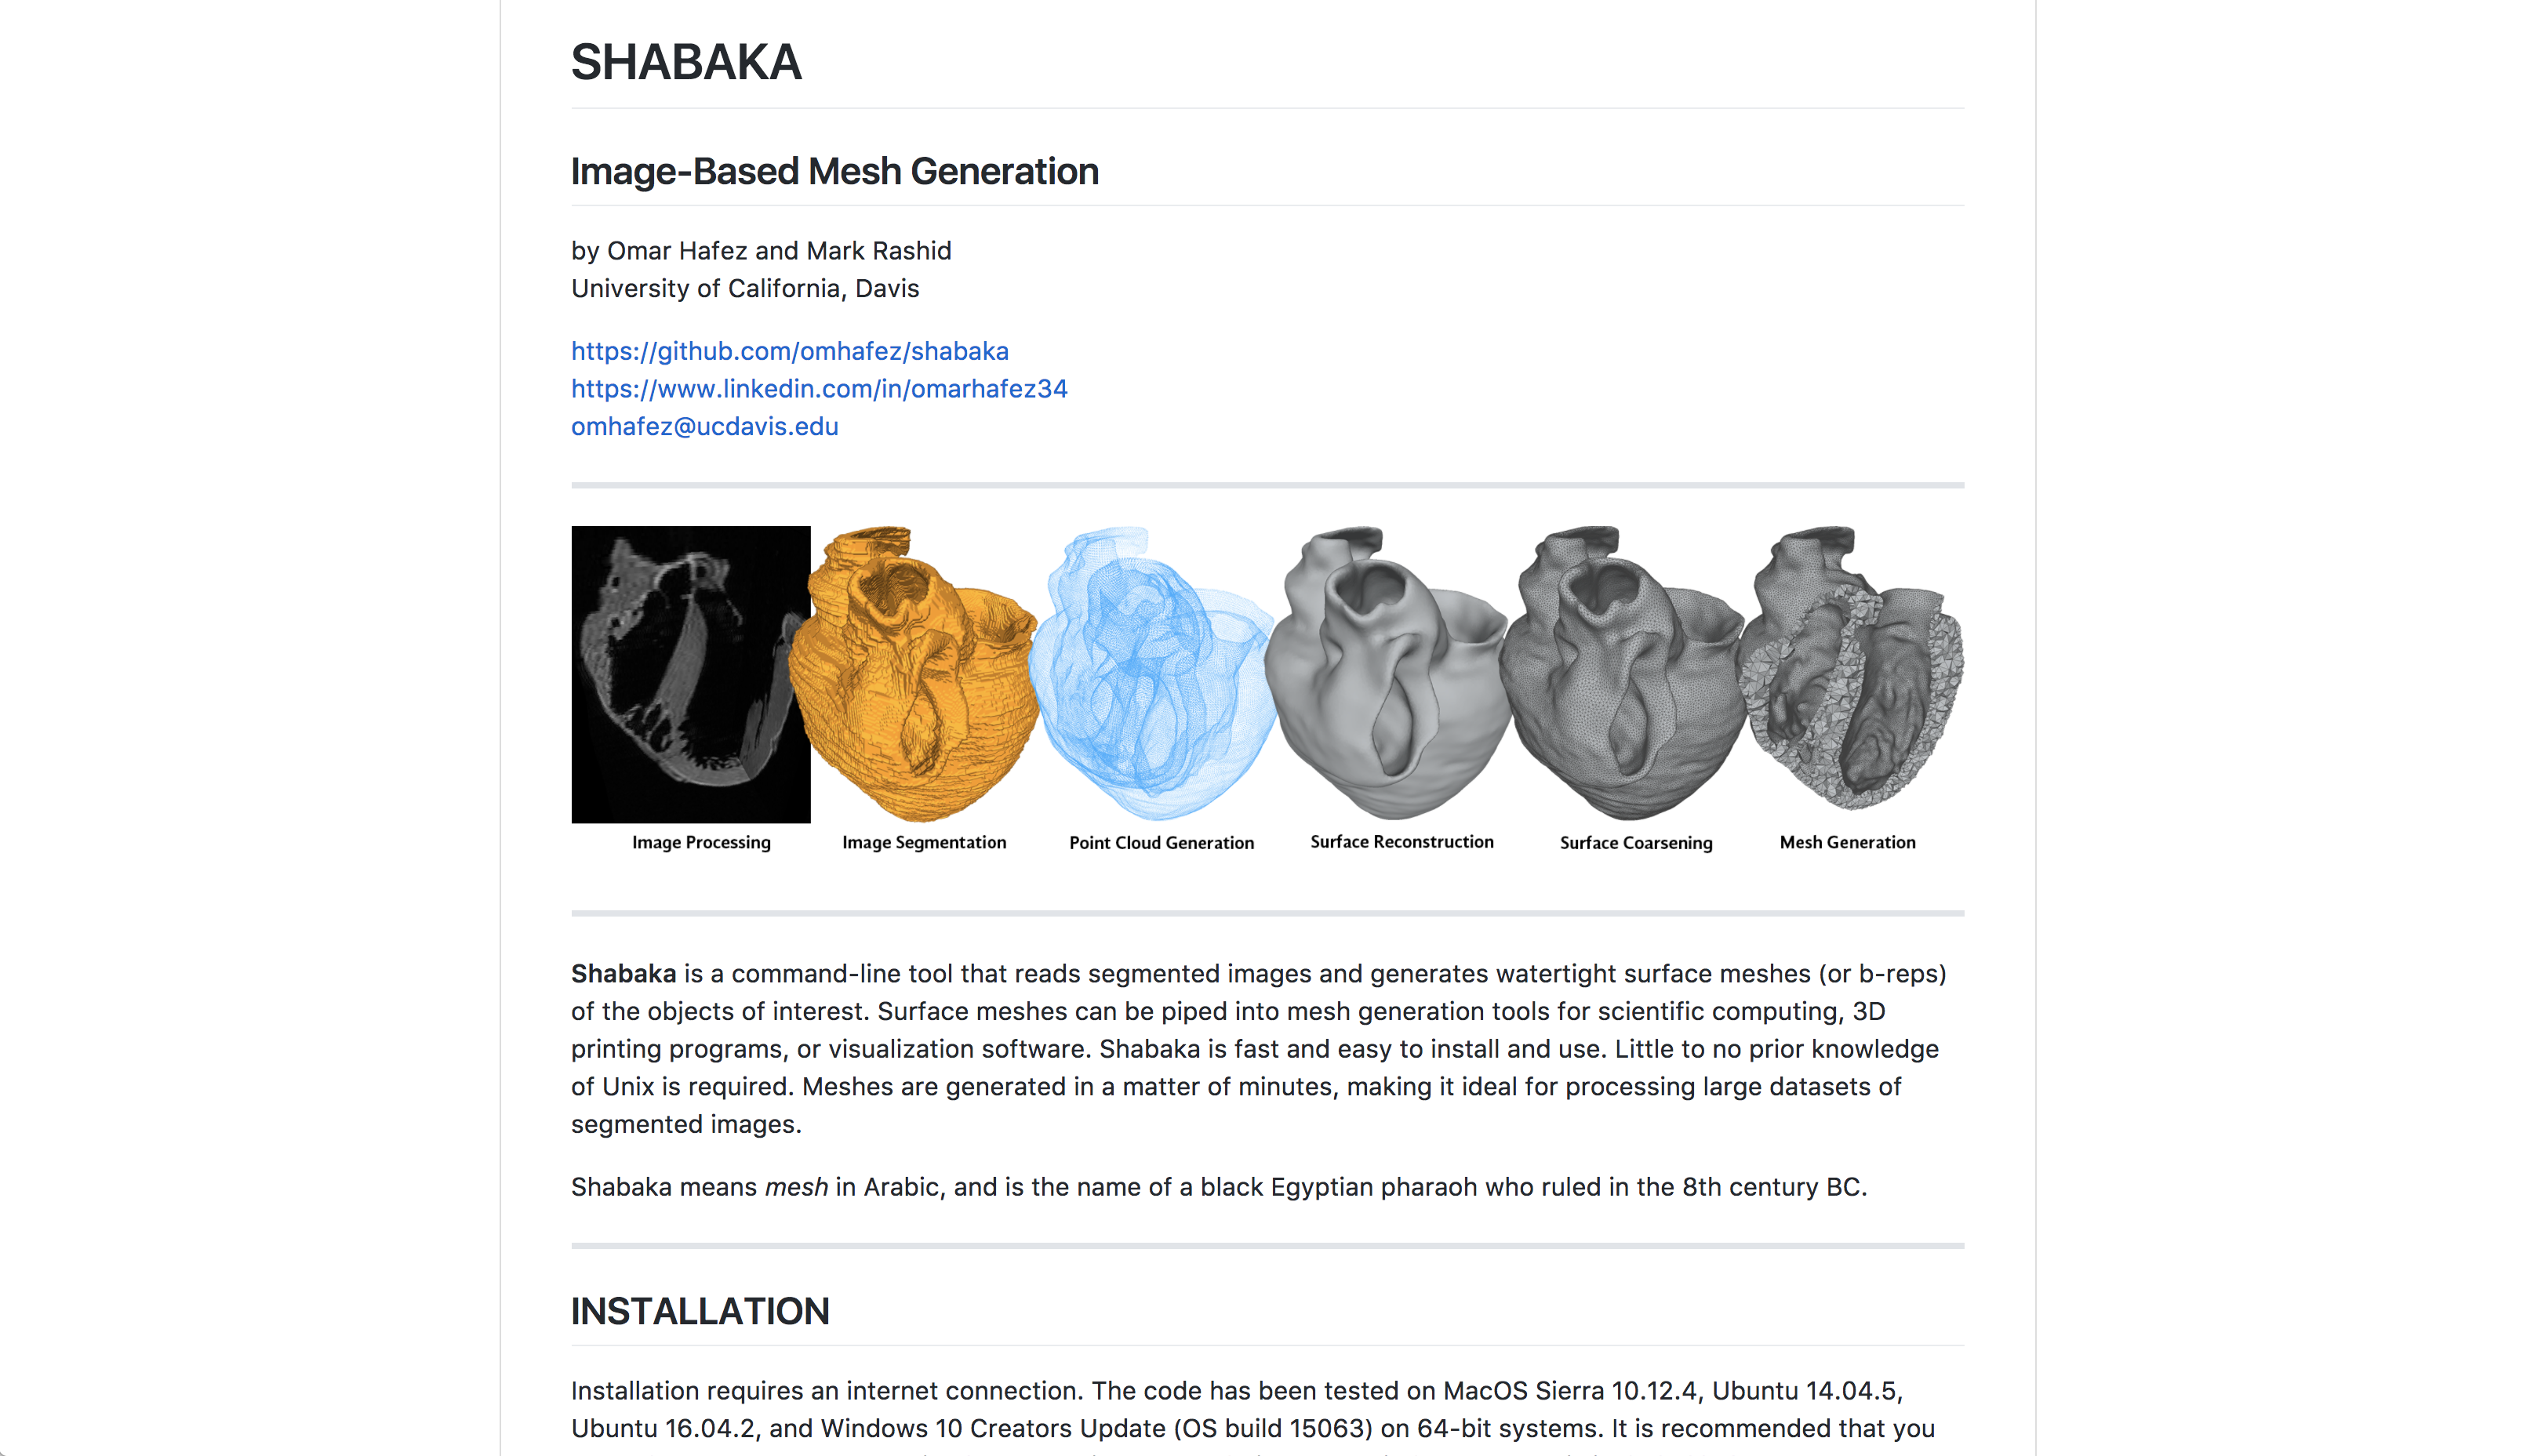
\includegraphics[width=1.0\textwidth]{media/2-shabaka/2-surf/7-shabaka.png}
\caption{Screenshot of Github repo}
\label{fig:github}
\end{figure}

\begin{figure}[ht]
\centering
\subfigure[]{%
		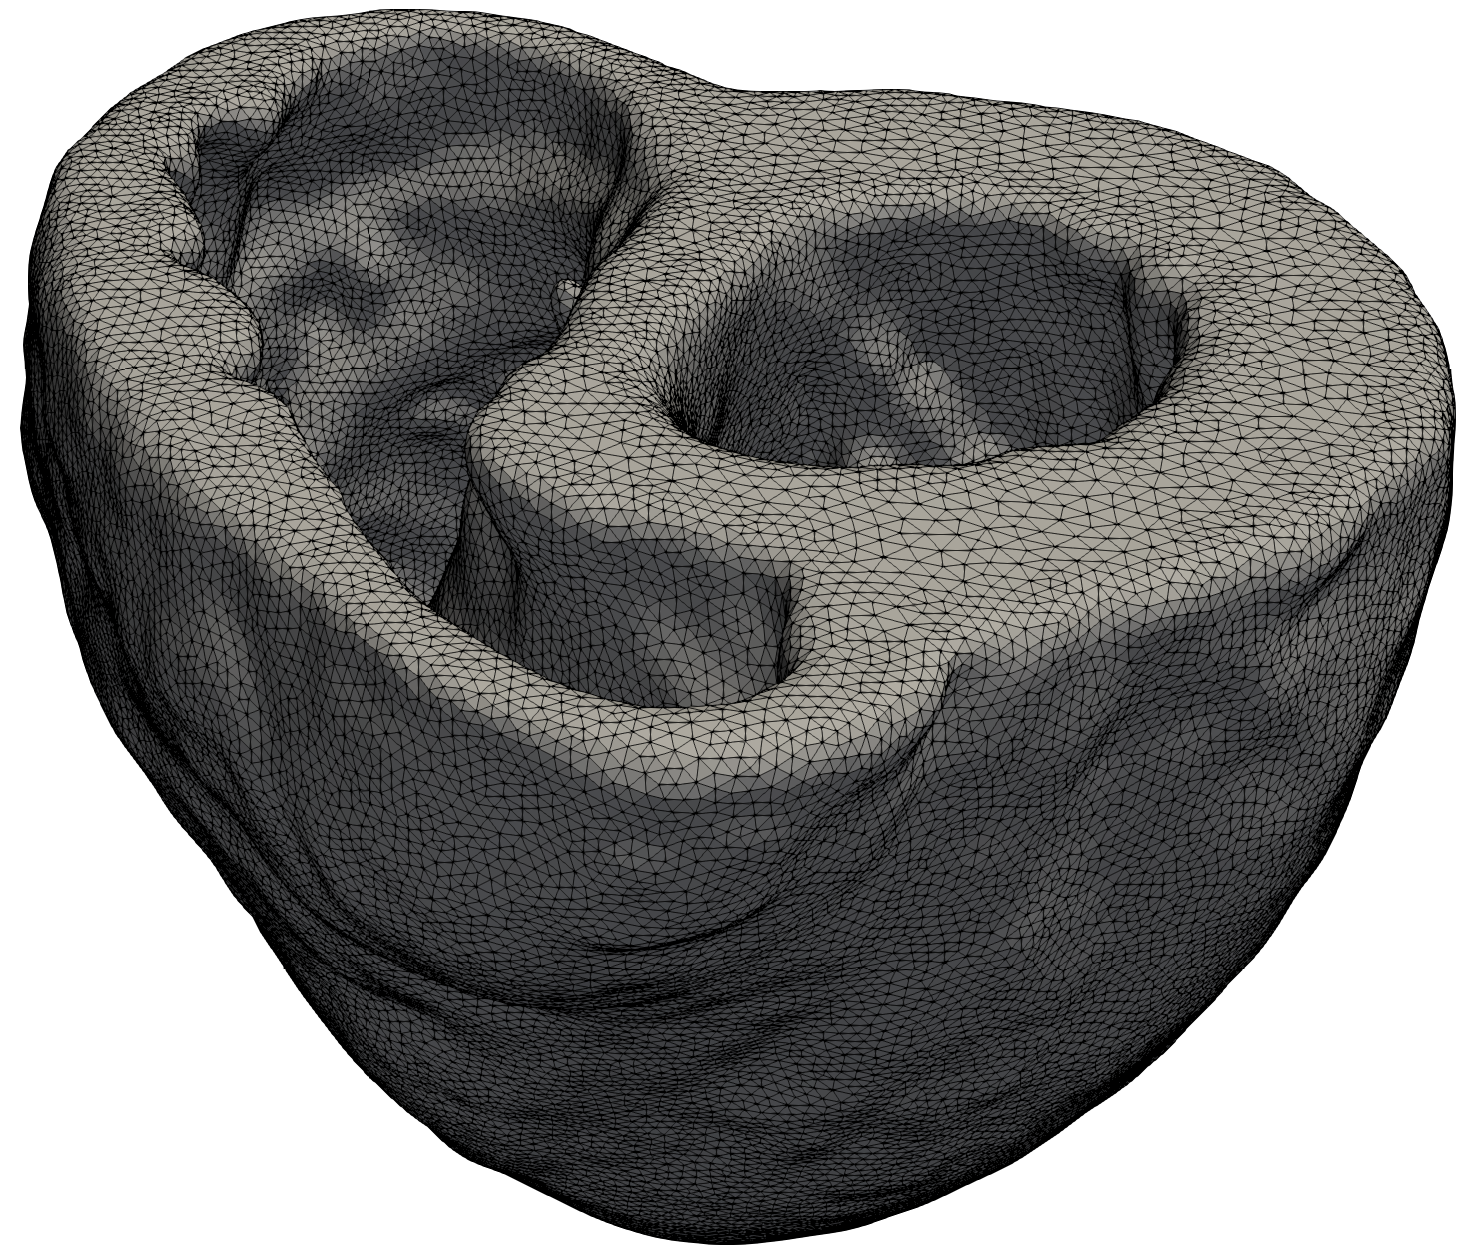
\includegraphics[scale=0.14]{media/4-cardioid/0-ventriclesurf.png}
\label{fig:tet1}}
\subfigure[]{%
		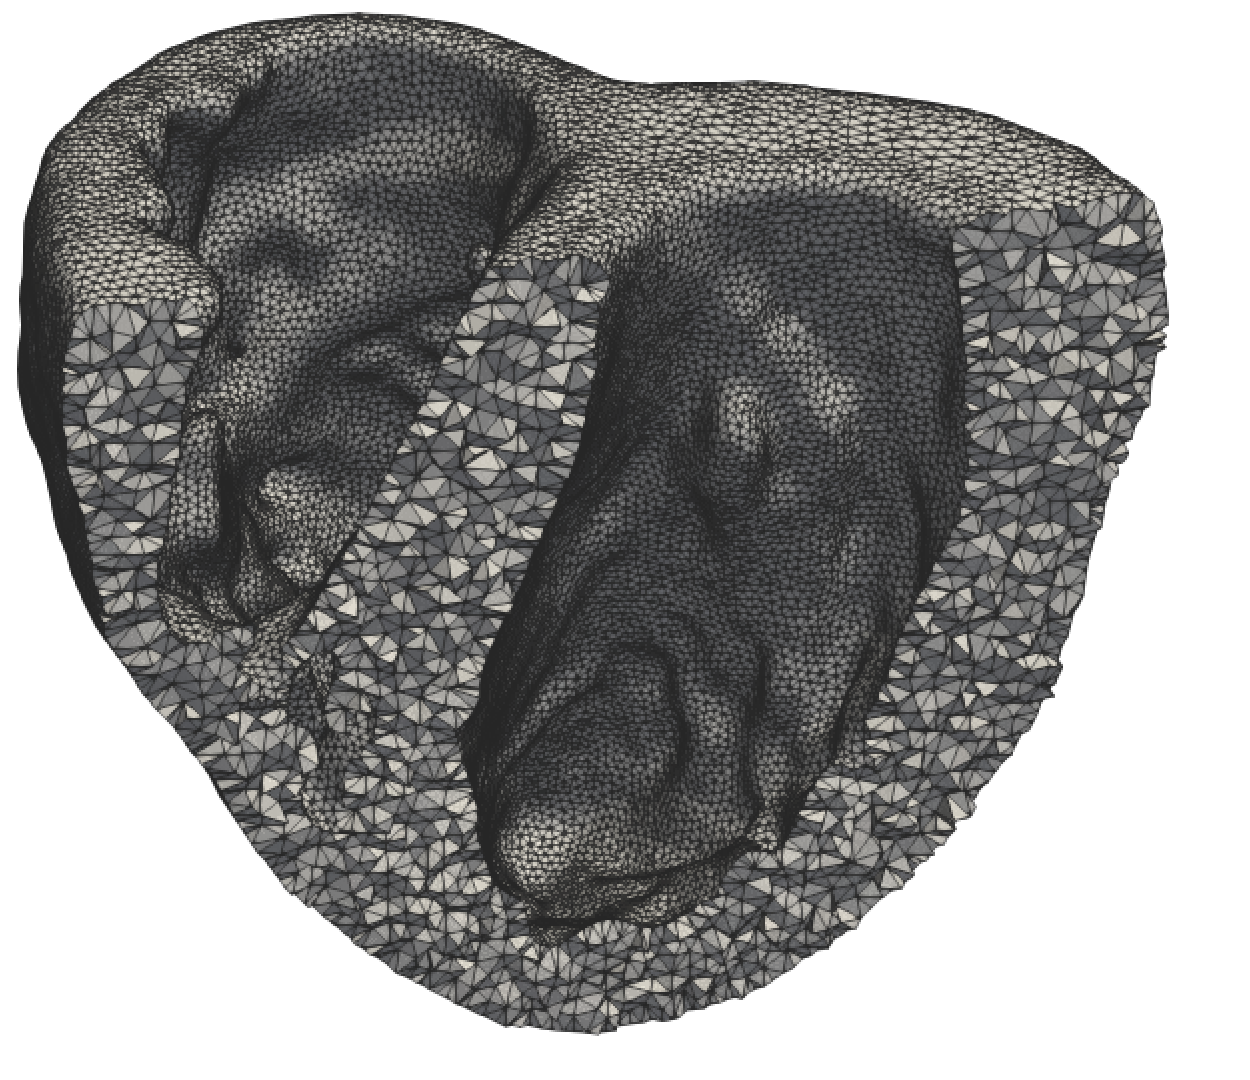
\includegraphics[scale=0.14]{media/4-cardioid/1-tet.png}
\label{fig:tet2}}
%
\caption{Bi-ventricular mesh: (a) surface mesh, and (b) clipped view of quadratic tetrahedral mesh used in Cardioid simulations}
\label{fig:tetmesh}
\end{figure}

\begin{figure}[ht]
\centering
\subfigure[]{%
		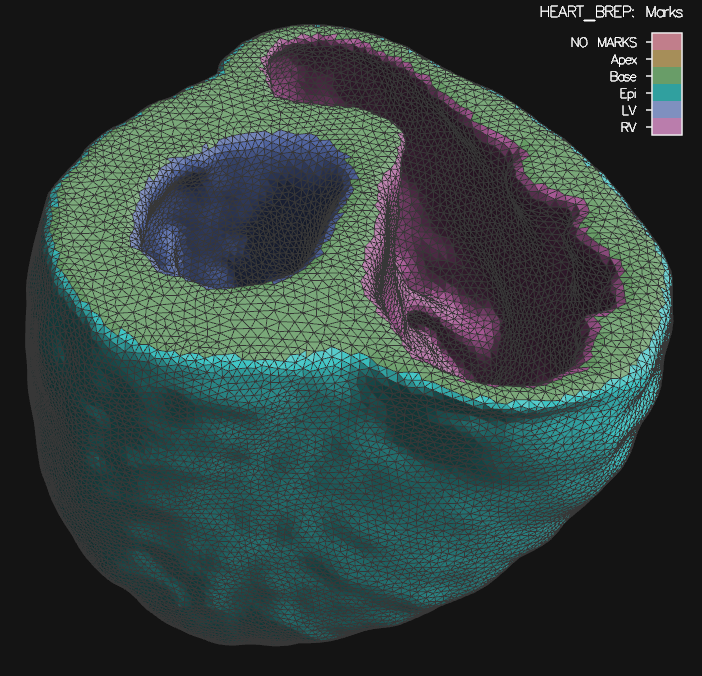
\includegraphics[scale=0.2]{media/3-celeris/1-brep.png}
\label{fig:cel1}}		
\subfigure[]{%
		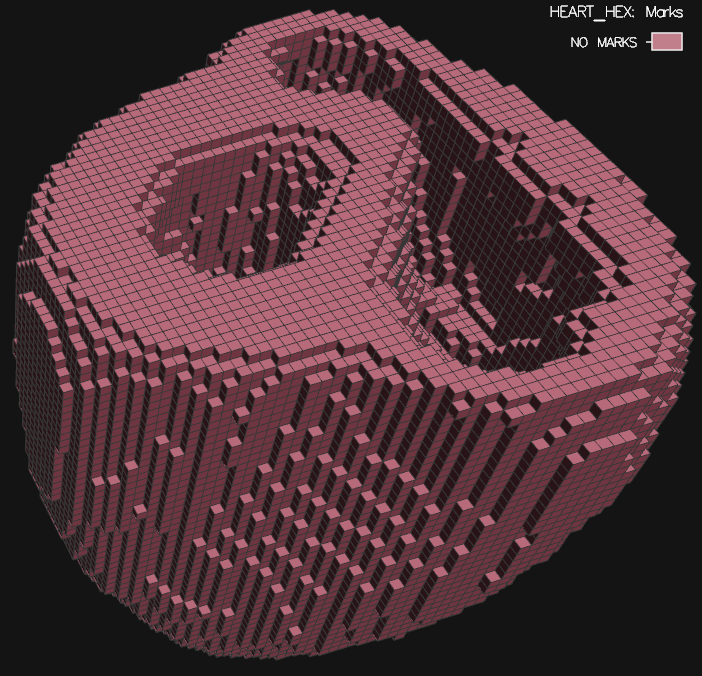
\includegraphics[scale=0.2]{media/3-celeris/2-hex.png}
\label{fig:cel2}}		
\subfigure[]{%
		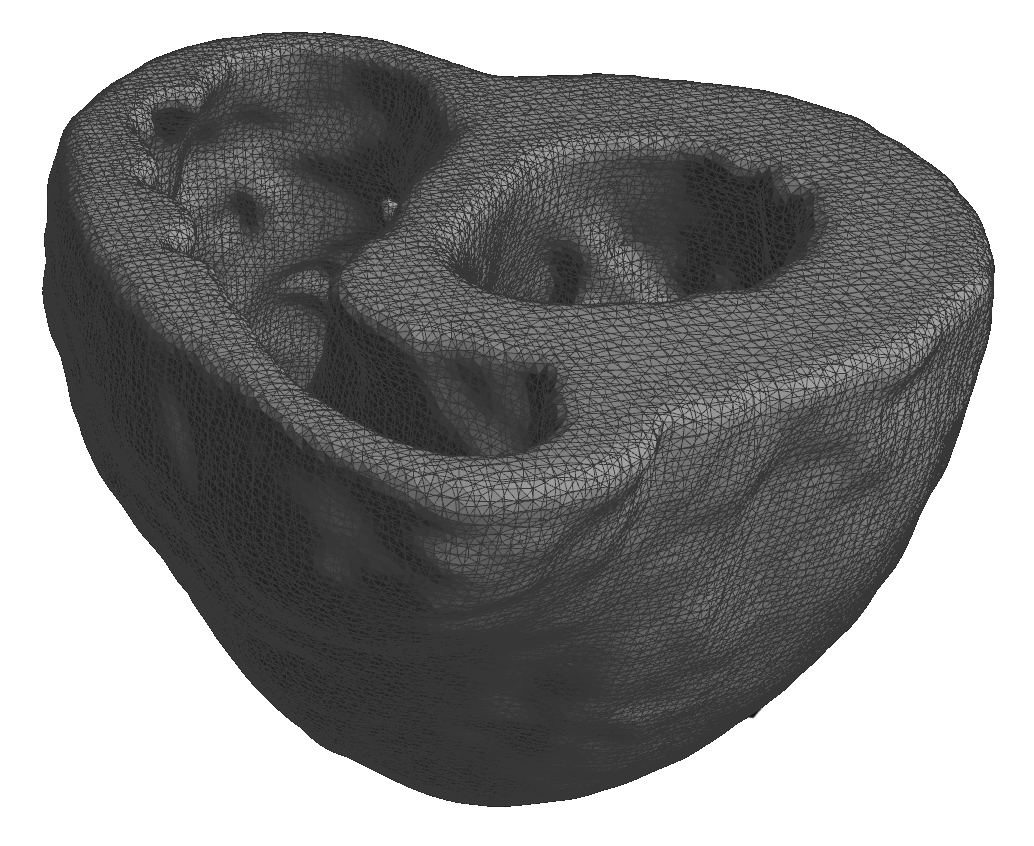
\includegraphics[scale=0.2]{media/3-celeris/3-pmesh.png}
\label{fig:cel3}}		
\subfigure[]{%
		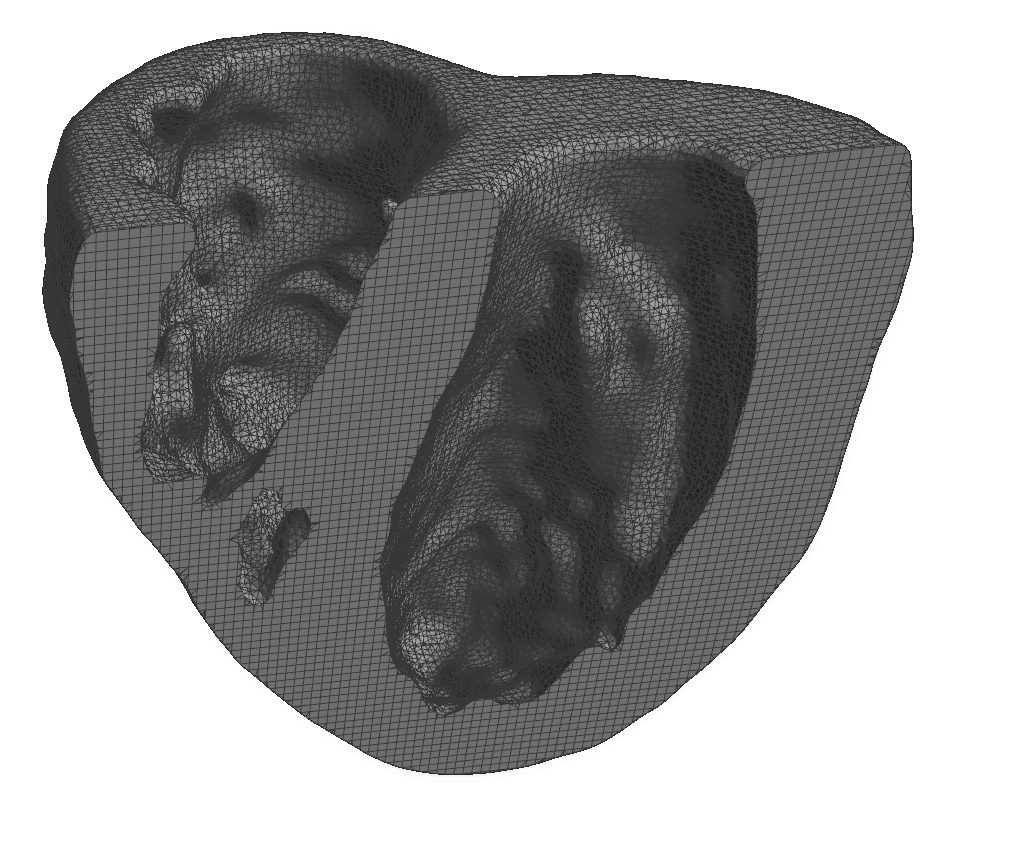
\includegraphics[scale=0.2]{media/3-celeris/4-clip.png}
\label{fig:cel4}}	
\subfigure[]{%
		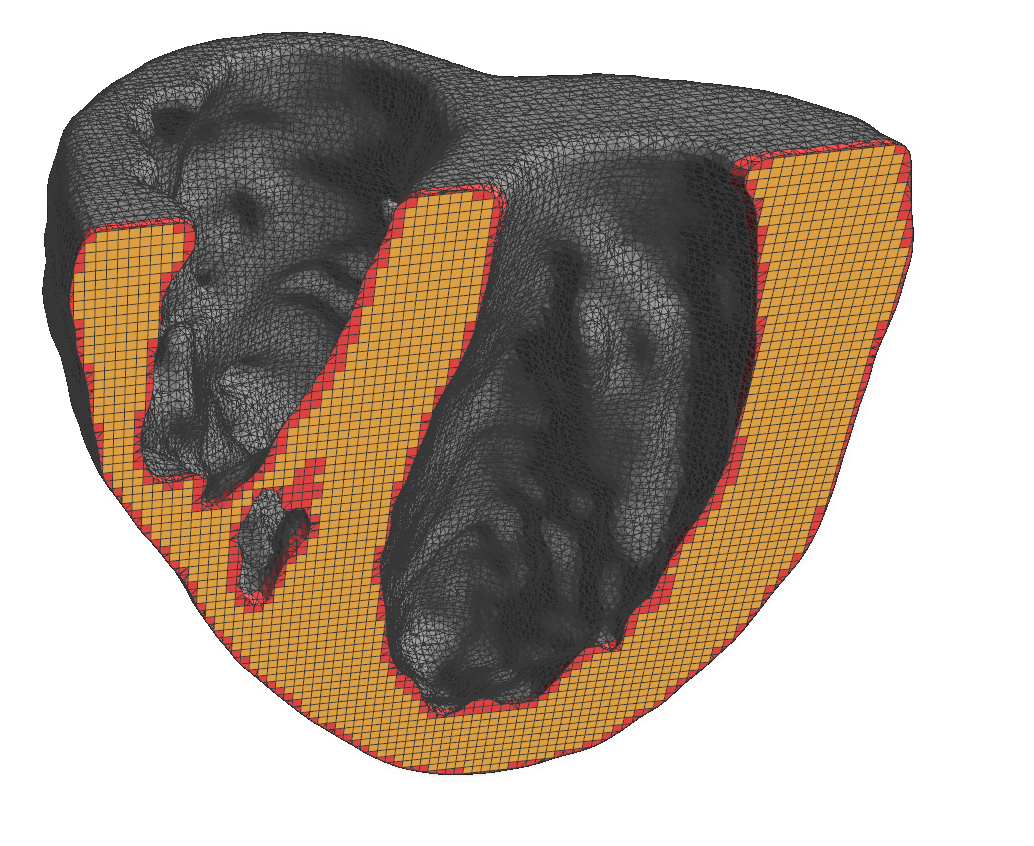
\includegraphics[scale=0.2]{media/3-celeris/5-color.png}
\label{fig:cel5}}			

\caption{Generation of polyhedral mesh: (a) input surface mesh, (b) bounding hex mesh,  (c) resulting polyhedral mesh, (d) clipped mesh, and (e) highlight of elements with cuboidal vs. general polyhedral shape.}
\label{fig:cel}
\end{figure}

\begin{figure}[ht]
\centering
\subfigure[]{%
		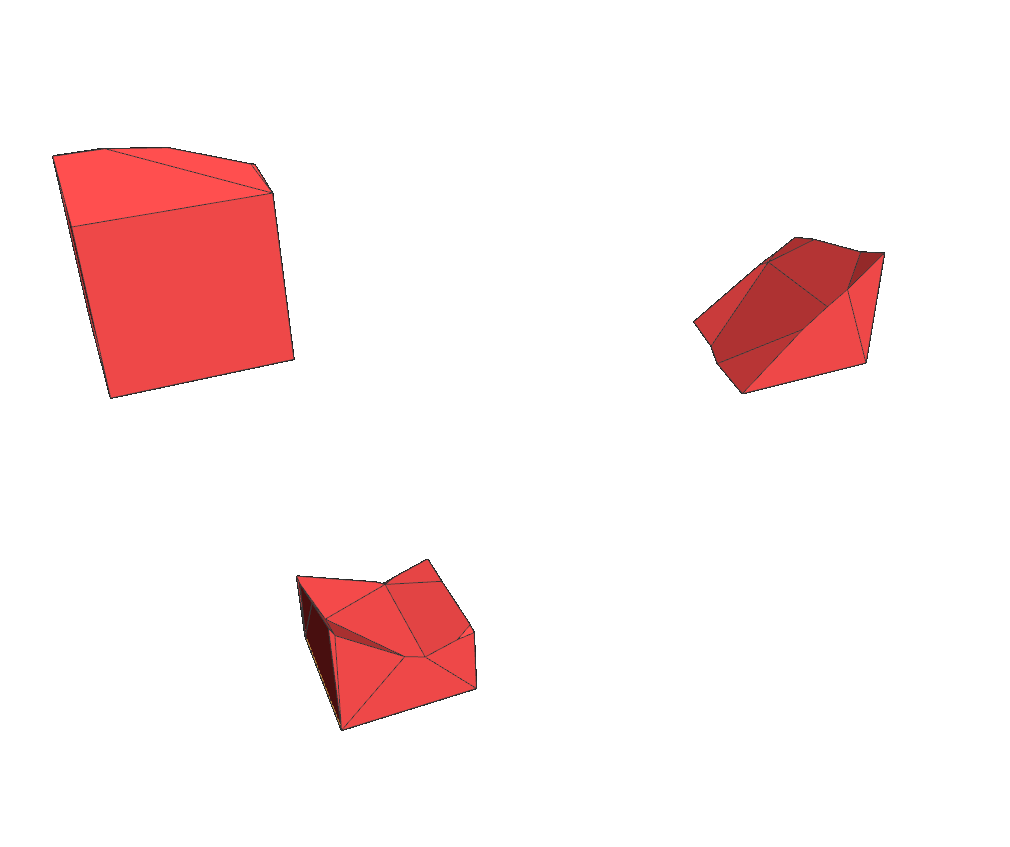
\includegraphics[scale=0.125]{media/3-celeris/zoom/zoom1.png}
\label{fig:zoom1}}		
\subfigure[]{%
		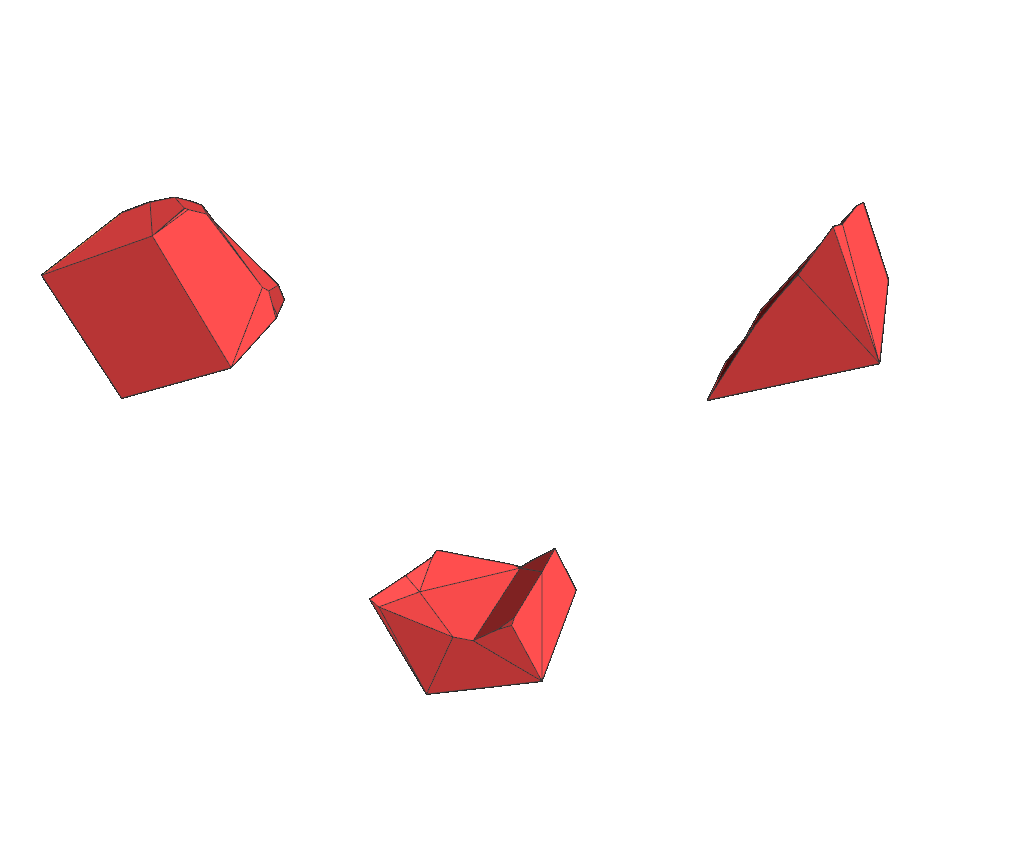
\includegraphics[scale=0.125]{media/3-celeris/zoom/zoom2.png}
\label{fig:zoom2}}		
\subfigure[]{%
		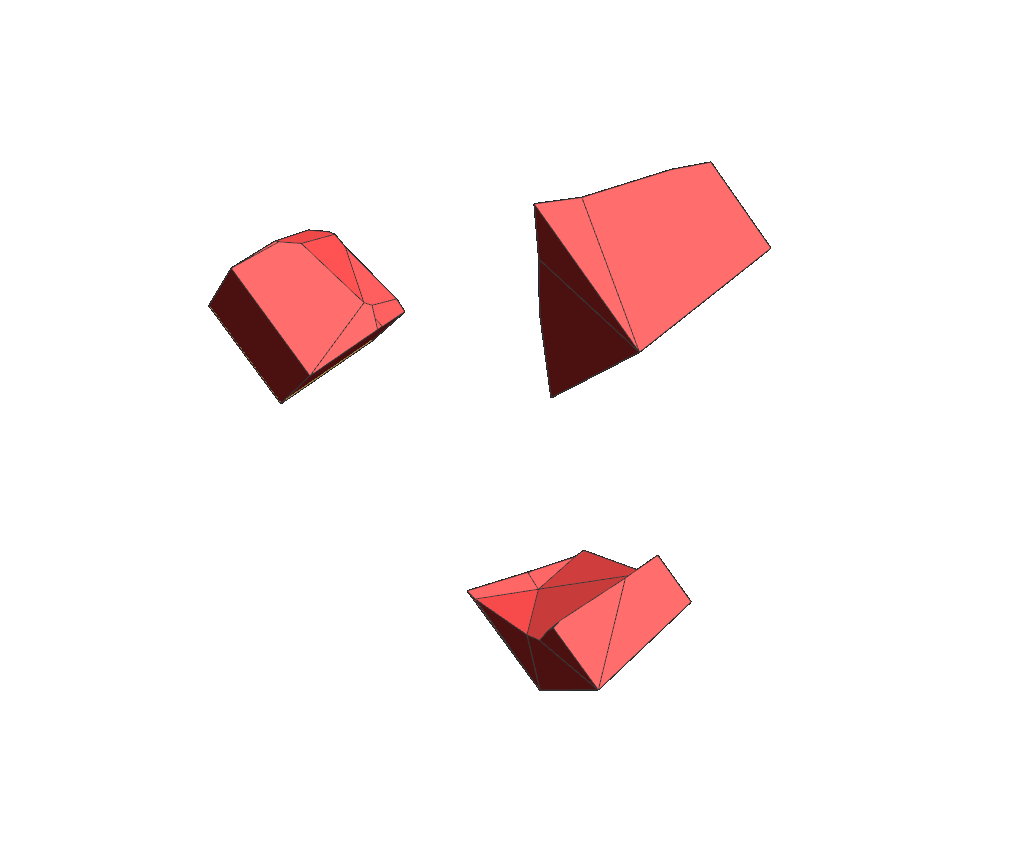
\includegraphics[scale=0.125]{media/3-celeris/zoom/zoom3.png}
\label{fig:zoom3}}		
\subfigure[]{%
		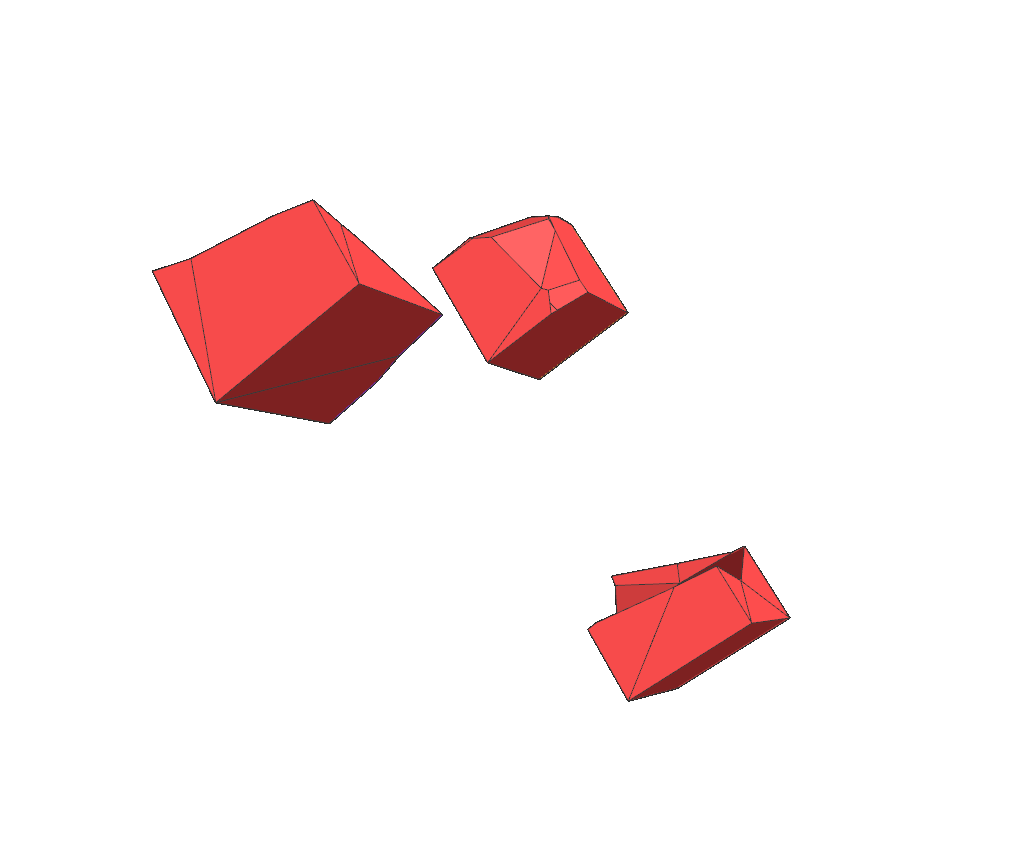
\includegraphics[scale=0.125]{media/3-celeris/zoom/zoom4.png}
\label{fig:zoom4}}	
\subfigure[]{%
		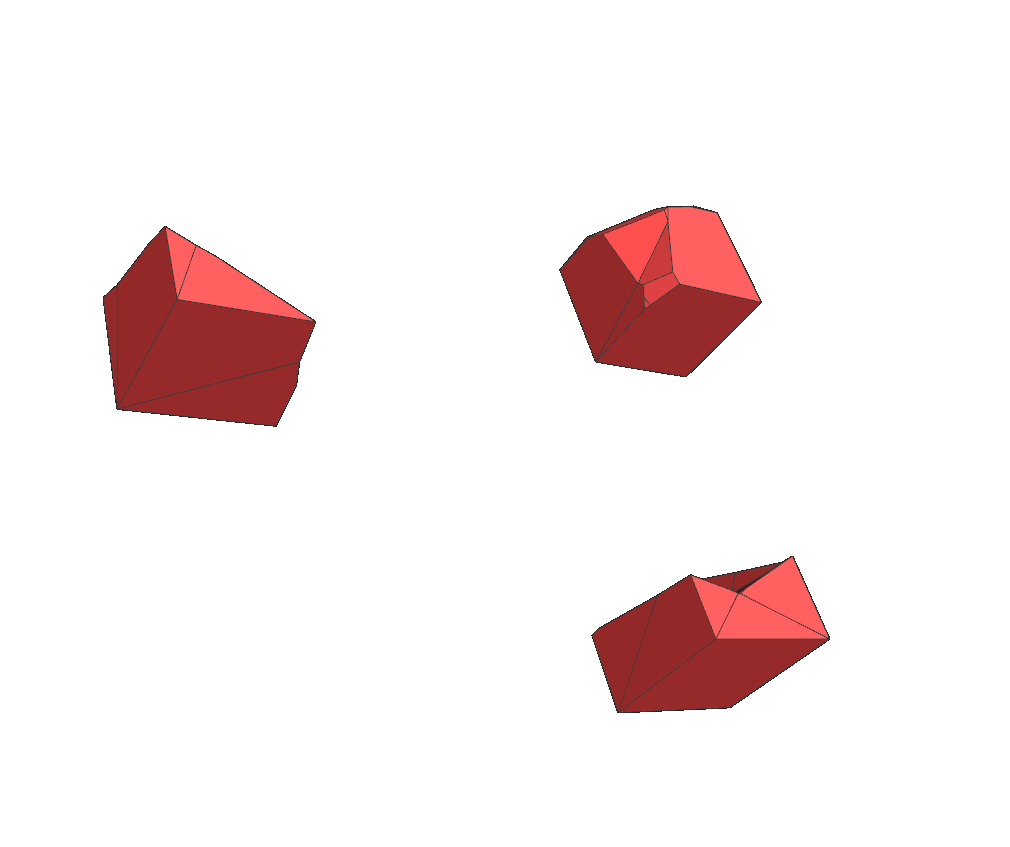
\includegraphics[scale=0.125]{media/3-celeris/zoom/zoom5.png}
\label{fig:zoom5}}		
\subfigure[]{%
		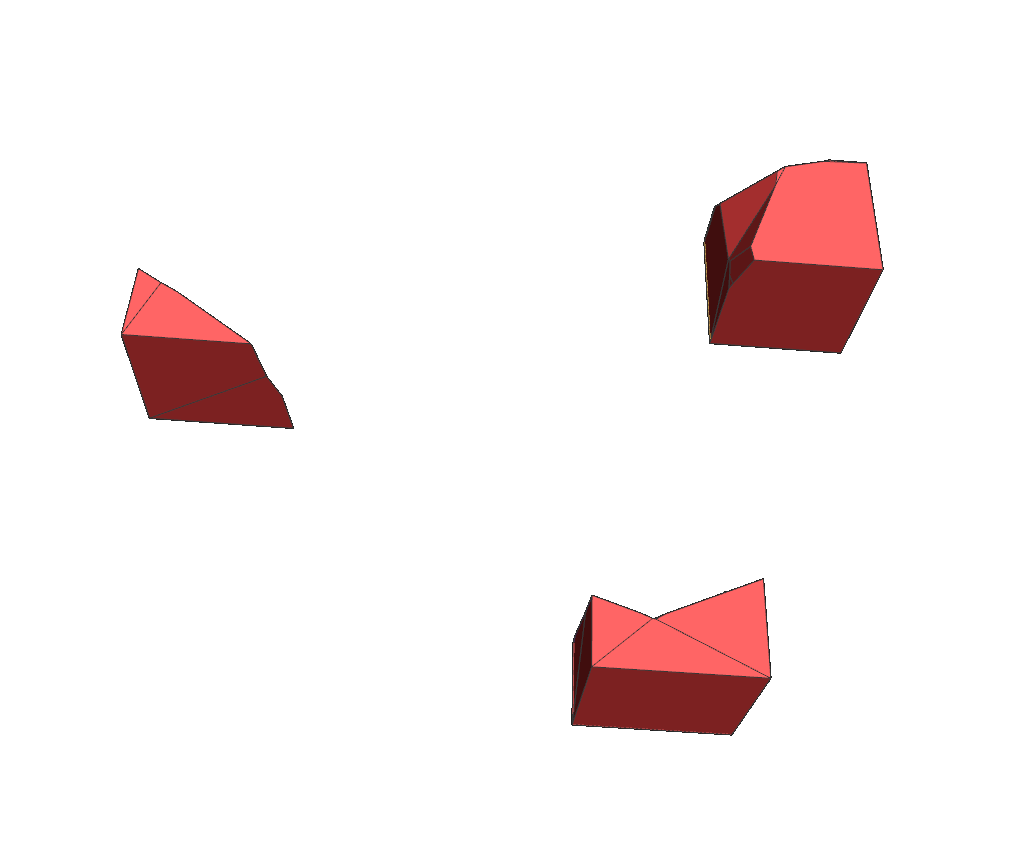
\includegraphics[scale=0.125]{media/3-celeris/zoom/zoom6.png}
\label{fig:zoom6}}	

\caption{Three example arbitrary polyhedral elements presented at different angles}
\label{fig:zoom}
\end{figure}

\begin{figure}[ht]
\centering
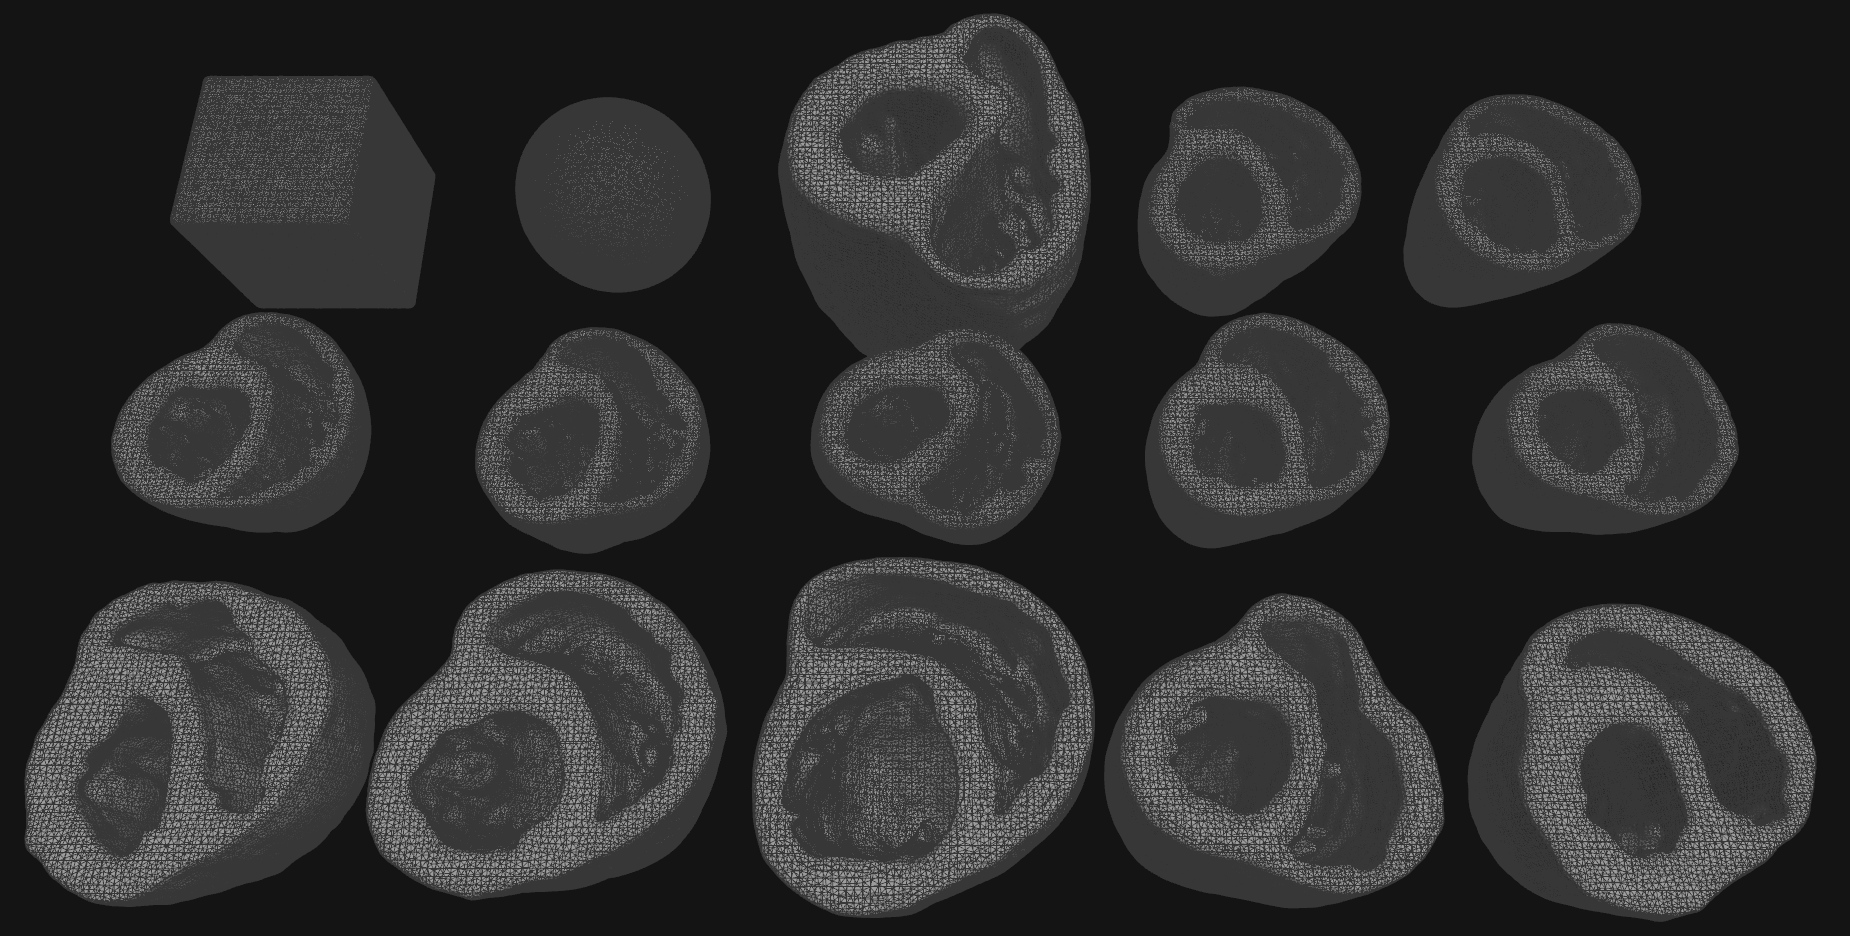
\includegraphics[width=1.0\textwidth]{media/3-celeris/7-suite.png}
\caption{Suite of polyhedral finite element meshes generated from image data \vspace{1cm}}
\label{fig:celsuite}
\end{figure}



%%%%%%%%%%%%%%%%%%%%%%%%%%%%%%%%%%%%%%%%%%%%%%%
%%%%%%%%%%%%%%%%%%%%%%%%%%%%%%%%%%%%%%%%%%%%%%%
\section{Review of Mesh Generation Techniques}
\label{Review of Mesh Generation Techniques}

Don't forget PhDResearch/doc/vorrecon \\

Hex meshing:
sweep mesh
thin sweep
multizone

Universal meshes for smooth surfaces with no boundary in three dimensions \\

Search Voronoi meshing from medical imaging. Or from segmented medical imaging

vmtk: http://www.vmtk.org/tutorials/ \\

http://www.robertschneiders.de/meshgeneration/software.html \\

$http://homepage.usask.ca/~ijm451/finite/fe_resources/mesh.html$ \\

- simpleware webinar \\

- downsampling - poisson disk sampling\\
- smooth normals\\
- filtering\\

- watertight surface reconstruction\\
	- vorocrust\\
	- powercrust\\
	- ball pivoting\\
	- poisson surface reconstruction\\
	- tight cocone\\
	
- meshing from CAD\\
    - tetgen\\
    - cubit/bolt\\
    
- direct meshing\\
	- simpleware\\

- smoothing after the fact\\
	- laplacian smooth\\

mesh simplification/decimation\\
cut cell approach\\
smoothing papers\\

noisy, oversampled point cloud\\


Simpleware webinar

- simpleware does not do CAD-based modeling, goes directly to the mesh
- contact regarding technical work/papers for meshing
export as STL, mesh, or NURBS
- TWO BOTTLENECKS
  - image segmentation time
  - generating watertight and error free meshes
    - no gaps or overlaps 
    - no inverted elements 
    - no negative jacobian
- segmentation -> stl -> smoothing -> nurbs -> meshing -  cad geometry medical device -> export final model -> poor elements, gaps and overlap, non convergence, not watertight
- manual corrections of stl, curbs, meshes

- generation of watertight STL
- aspect ratio/mesh quality
- image-based meshing

- BLENDR - graphics, STL
- Rhino - STL generation, NURBS

Email Kerim, k.genc@simpleware.com

see you at WCCM
Ross Cotton’s recently published paper
Ross Cotton, r.cotton@simpleware.com

Simpleware paper:
1. marching cubes for surface mesh
2. Advancing front or Delaunay techniques for tet meshing --> produces slivers though
3. Extended EVoMacs

hex meshers:

truegrid\\
cubit

mask to mesh:
dual contouring

"state of the art" papers\\
Sculpt Sandia - grid based meshing, volume fraction \\
"Parallel hex meshing from volume fractions"\\
For each voxel, sample a bunch of points, decide if inside or outside \\
Look at neighboring cells, do least squares to approximate gradient and throw down normal \\

Netgen advancing front. Mimix hex mesher \\

Truegrid hex mesher \\
CUBIT \\
Mimix \\

automated hex meshing at uconn: http://im.engr.uconn.edu/downloads.php


SURFACE RECONSTRUCTION:
show results from Poison surf recon, powercrust, tight cocone \\

SimVascular: 2D segmentations followed by lofting



DECIMATION/SURFACE COARSENING:\\
ACVD papers
Quadric Edge-Collapse Decimation

%%%%%%%%%%%%%%%%%%%%%%%%%%%%%%%%%%%%%%%%%%%%%%%
%%%%%%%%%%%%%%%%%%%%%%%%%%%%%%%%%%%%%%%%%%%%%%%
\section{Voronoi Partitioning}
\label{Voronoi Partitioning}
Voro++

%%%%%%%%%%%%%%%%%%%%%%%%%%%%%%%%%%%%%%%%%%%%%%%
%%%%%%%%%%%%%%%%%%%%%%%%%%%%%%%%%%%%%%%%%%%%%%%
\section{Tolerance-Aware Voronoi Partitioning}
\label{Tolerance-Aware Voronoi Partitioning}
%%%%%%%%%%%%%%%%%%%%%%%%%%%%%%%%%%%%%%%%%%%%%%%
%%%%%%%%%%%%%%%%%%%%%%%%%%%%%%%%%%%%%%%%%%%%%%%
\section{Voronoi-Based Mesh Generation}
\label{Voronoi-Based Mesh Generation}
%%%%%%%%%%%%%%%%%%%%%%%%%%%%%%%%%%%%%%%%%%%%%%%
%%%%%%%%%%%%%%%%%%%%%%%%%%%%%%%%%%%%%%%%%%%%%%%
\section{Boundary Representation (B-rep) Generation}
\label{Boundary Representation (B-rep) Generation}
%%%%%%%%%%%%%%%%%%%%%%%%%%%%%%%%%%%%%%%%%%%%%%%
%%%%%%%%%%%%%%%%%%%%%%%%%%%%%%%%%%%%%%%%%%%%%%%
\section{Robust Polyhedral Mesh Generation from B-reps}
\label{Robust Polyhedral Mesh Generation from B-reps}

\chapter{Modeling \& Simulation}
%


%%%%%%%%%%%%%%%%%%%%%%%%%%%%%%%%%%%%%%%%%%%%%%%
%%%%%%%%%%%%%%%%%%%%%%%%%%%%%%%%%%%%%%%%%%%%%%%
\section{Continuum Mechanics}
\label{Continuum Mechanics}
%%%%%%%%%%%%%%%%%%%%%%%%%%%%%%%%%%%%%%%%%%%%%%%
%%%%%%%%%%%%%%%%%%%%%%%%%%%%%%%%%%%%%%%%%%%%%%%
\section{The Finite Element Method}
\label{The Finite Element Method}
(refer also to Jeremic and Felippa lecture notes, and Tom Hughes book)
%%%%%%%%%%%%%%%%%%%%%%%%%%%%%%%%%%%%%%%%%%%%%%%
%%%%%%%%%%%%%%%%%%%%%%%%%%%%%%%%%%%%%%%%%%%%%%%
\section{Incremental Kinematics}
\label{Incremental Kinematics}
see celeris/doc/NLmat.pdf
%%%%%%%%%%%%%%%%%%%%%%%%%%%%%%%%%%%%%%%%%%%%%%%
%%%%%%%%%%%%%%%%%%%%%%%%%%%%%%%%%%%%%%%%%%%%%%%
\section{Hyperelastic Materials}
\label{Hyperelastic Materials}
%%%%%%%%%%%%%%%%%%%%%%%%%%%%%%%%%%%%%%%%%%%%%%%
%%%%%%%%%%%%%%%%%%%%%%%%%%%%%%%%%%%%%%%%%%%%%%%
\section{The Partitioned Element Method}
\label{The Partitioned Element Method}

https://gaoxifeng.github.io/research.html \\
https://github.com/gaoxifeng/robust_hex_dominant_meshing

%%%%%%%%%%%%%%%%%%%%%%%%%%%%%%%%%%%%%%%%%%%%%%%%%%%%%%%%%%%%%%%%%%%%%%%%%%%%%%%%%%%%%%%%%%%%%%%%%%%%%%%%
%%%%%%%%%%%%%%%%%%%%%%%%%%%%%%%%%%%%%%%%%%%%%%%%%%%%%%%%%%%%%%%%%%%%%%%%%%%%%%%%%%%%%%%%%%%%%%%%%%%%%%%%

\chapter{Application: Cardiac Mechanics}
%

Cardioid science on saturday Youtube
$heart_papers$
papers Mark mentions in SOW

%%%%%%%%%%%%%%%%%%%%%%%%%%%%%%%%%%%%%%%%%%%%%%%
%%%%%%%%%%%%%%%%%%%%%%%%%%%%%%%%%%%%%%%%%%%%%%%
\section{Description of Cardioid}
\label{Description of Cardioid}

%%%%%%%%%%%%%%%%%%%%%%%%%%%%%%%%%%%%%%%%%%%%%%%
%%%%%%%%%%%%%%%%%%%%%%%%%%%%%%%%%%%%%%%%%%%%%%%
\section{Material Property Characterization}
\label{Material Property Characterization}

%%%%%%%%%%%%%%%%%%%%%%%%%%%%%%%%%%%%%%%%%%%%%%%
%%%%%%%%%%%%%%%%%%%%%%%%%%%%%%%%%%%%%%%%%%%%%%%
\section{Fiber Generation}
\label{Simulation}

%%%%%%%%%%%%%%%%%%%%%%%%%%%%%%%%%%%%%%%%%%%%%%%
%%%%%%%%%%%%%%%%%%%%%%%%%%%%%%%%%%%%%%%%%%%%%%%
\section{Boundary Conditions}
\label{Boundary Conditions}

%%%%%%%%%%%%%%%%%%%%%%%%%%%%%%%%%%%%%%%%%%%%%%%
%%%%%%%%%%%%%%%%%%%%%%%%%%%%%%%%%%%%%%%%%%%%%%%
\section{Simulation/Results}
\label{Simulation/Results}


Questions to ask with available model
Effect of smoothing/trabeculae
Do trabeculae affect the solution
How sensitive are the results from paraview smoothing?
Effect of resolution – make multiple meshes of same geometry
Number of iterations – do they depend on mesh resolution? Would like it not to 
Does V cycle work for my geometry?
Fiber generation vs fibers from raw data + interp + smoothing
Verification/validation
Stress/strain plots
Initial cycle is faster than others: first frame but also first cycle all together is faster
Mesh quality/aspect ratio
Potential plots:	
Volumetric strain
Deviatoric strain
C11, c22, c33
Maximal principal eigenvalue
C11 from fiber orientation
Hysteresis plot of position

structure/trabeculae
fibergen vs DTI
Jeremy drug studies, a lot didn’t match
whole range of sensitivity studies

\chapter{Discussion}
%

\section{Future Work}
\label{Future Work}
%%%%%%%%%%%%%%%%%%%%%%
%%%%%%%%%%%%%%%%%%%%%%
\section{Towards Automating the Image-to-Analysis Pipeline}
\label{Towards Automating the Image-to-Analysis Pipeline}
%%%%%%%%%%%%%%%%%%%%%%
%%%%%%%%%%%%%%%%%%%%%%
\subsection{Multiple Materials and Inhomogeneous Materials}
\label{Multiple Materials and Inhomogeneous Materials}
%%%%%%%%%%%%%%%%%%%%%%
%%%%%%%%%%%%%%%%%%%%%%
\subsection{Uncertainty Quantification, Verification, and Validation}
\label{Uncertainty Quantification, Verification, and Validation}
Material properties, boundary conditions
%%%%%%%%%%%%%%%%%%%%%%
%%%%%%%%%%%%%%%%%%%%%%
\subsection{High Performance Computing}
\label{High Performance Computing}
%%%%%%%%%%%%%%%%%%%%%%
%%%%%%%%%%%%%%%%%%%%%%
\section{Clinical Implications}
\label{Clinical Implications}
(haptics, Simpleware stuff)\\
Center for Cardiovascular simulation (Texas)
Heartflow, Inc., Charles Taylor

ASME V\&V10 and V\&V40

dental applications - 1) for implant placement and crown design, 2) for 3D printing, aesthetic try-in 

tolerance-aware voronoi-partitioning \\
multiple material interfaces (see paper) \\

Abaqus: ability to deal with initial over-closures? A strain-free adjustment perhaps? Like if you were to mesh the femur and the femoral cartilage separately, say, and there is a tiny bit of overlap between them..are you able to fix this without going back to the meshing software?
\chapter{Future Work}
%



\chapter{Appendix: Glossary of Terms}
%




\bibliography{references}

% The UMI abstract uses square brackets!
\UMIabstract[The abstract that is submitted to UMI must be formatted as shown in the example here. The body of the abstract cannot exceed 350 words. It should be in typewritten form, double-spaced, and on bond paper. It is important to write an abstract that gives a clear description of the content and major divisions of the dissertation, since UMI will publish the abstract exactly as submitted. Students completing their requirements under Plan A should provide extra copies of the typed summary for use by the dissertation committee during the examination.

The abstract that is submitted to UMI must be formatted as shown in the example here. The body of the abstract cannot exceed 350 words. It should be in typewritten form, double-spaced, and on bond paper. It is important to write an abstract that gives a clear description of the content and major divisions of the dissertation, since UMI will publish the abstract exactly as submitted. Students completing their requirements under Plan A should provide extra copies of the typed summary for use by the dissertation committee during the examination.

The abstract that is submitted to UMI must be formatted as shown in the example here. The body of the abstract cannot exceed 350 words. It should be in typewritten form, double-spaced, and on bond paper. It is important to write an abstract that gives a clear description of the content and major divisions of the dissertation, since UMI will publish the abstract exactly as submitted. Students completing their requirements under Plan A should provide extra copies of the typed summary for use by the dissertation committee during the examination.

The abstract that is submitted to UMI must be formatted as shown in the example here. The body of the abstract cannot exceed 350 words. It should be in typewritten form, double-spaced, and on bond paper. It is important to write an abstract that gives a clear description of the content and major divisions of the dissertation, since UMI will publish the abstract exactly as submitted. Students completing their requirements under Plan A should provide extra copies of the typed summary for use by the dissertation committee during the examination.]

\end{document} 